\chapter{\label{viterbi}Viterbi Search}

To search for \ac{CW} signals, an adaptation of the Viterbi algorithm, which is well known in telecommunications, is used to search through spectrograms of \ac{LIGO} data. The basic idea of the search is simple, if we looked at a spectrogram frequency band as in Fig.~\ref{} we could find every possible track from a starting frequency bin to an end frequency bin (of which there are many). For each of these tracks the sum of the sprectrogram power along the track can be found such that for each track there is a single value, Fig.~\ref{} shows a histogram of these values. If there is a signal present in this band then it could be  assumed that the signal which gives the highest sum of spectrogram power is the track which is most likely to follow the signals frequency track.
Therefore, it can be assumed that if the frequency track with the highest sum of spectrogram power is found, then the corresponding track is most likely for follow a signal. 
Now as calculating all possible tracks is time consuming and the majority of tracks will not follow the signal track, it woudl be useful to have an algorithm which could find the maximum track more efficiently. This is where the Viterbi algorithm \cite{Viterbi} does this exact task. This is explained in the following sections.

\section{Viterbi algorithm}
%
% Into to viterbi
%
The Viterbi algorithm is an efficient method for determining the most probable set of states (a single `track' of steps on the time-frequency plane) in a Markov model dependent on data, where the model has a discrete number of states at each step. Rather than computing the probability of every possible track and selecting the most probable, the algorithm maximises this probability after every discrete step. As a result, a partial track which cannot ultimately be the most probable is rejected before the next step is calculated, and only a fraction of all possible tracks need to be computed to find the one that is most probable.

%
% Defining varibles and what data we use
%
In this work we apply the Viterbi algorithm to a \ac{GW} strain time-series to find the most probable track of a single variable-frequency signal in the noisy data.  We divide the time series into $N$ equal-length and contiguous segments ${\bm x}_j$,  defining the set $D \equiv \{{\bm x}_j\}$. The `states' in the model correspond to the frequencies a signal could have in each segment. A `track' is a list of such frequencies ${\bm \nu}\equiv \{\nu_j\}$, where  $\nu_j$ is the frequency in the segment ${\bm x_j}$.

%
% defining probabilities
%
Our objective is to calculate the most probable track given the data, i.e., the
track that maximises $p({\bm \nu}\mid D)$. Using Bayes theorem, this posterior probability can
be written as
%
\begin{equation}
\label{viterbi:bayes}
  p({\bm \nu} \mid D) = \frac{p({\bm \nu})p(D \mid {\bm \nu})}{p(D)},
\end{equation}
%
where $p({\bm \nu}) $ is the prior probability of the
track, $p(D \mid{\bm \nu})$ is the likelihood of the track (i.e., the
probability of the data given the track) and $p(D)$ is the model evidence (or
marginalised likelihood).

The Viterbi algorithm treats the track as the result of a Markovian process,
such that the current state depends only on the previous state. It is
therefore useful to split the track's prior into a set of transition
probabilities such that
%
\begin{align}
\label{viterbi:prior}
p({\bm \nu}) &= p(\nu_{N - 1}, \ldots, \nu_1, \nu_0)\nonumber \\
%&=  p(\omega_{N} \mid \omega_{N-1}, \ldots, \omega_1,\omega_0)p(\omega_{N-1} \mid \omega_{N-2}, \ldots, \omega_1,\omega_0) \ldots p(\omega_1 \mid \omega_0)p(\omega_0) \\
&= p(\nu_{N - 1} \mid \nu_{N-2})p(\nu_{N-2} \mid \nu_{N-3}) \dots p(\nu_1 \mid \nu_0)p(\nu_0) \nonumber \\
&= p(\nu_0)\prod_{j=1}^{N-1}p(\nu_{j} \mid \nu_{j-1}),
\end{align}
%
where $p(\nu_0)$ is the prior probability that the signal in the first time
step has a frequency $\nu_0$ and $p(\nu_{j} \mid \nu_{j-1})$ is the
prior `transition' probability for $\nu_j$ given the frequency at the last
step was $\nu_{j-1}$.

The noise in each of the segments can be treated as independent, so the
likelihood component in Eq.~\ref{viterbi:bayes} can be factorised as
%
\begin{equation}
\label{viterbi:likelihood}
p(D \mid {\bm \nu}) = \prod_{j=0}^{N-1}p({\bm x_j} \mid \nu_j),
\end{equation}
%
 where $p({\bm x_j} \mid \nu_j)$ is the likelihood of our
signal having a frequency $\nu_j$ in the $j$th segment.

Using Eqs.~\ref{viterbi:bayes},\ref{viterbi:prior} and
\ref{viterbi:likelihood}, the posterior probability is then
%
\begin{equation}
\label{viterbi:posterior}
    p({\bm \nu} | D) =
    \frac{p(\nu_0)p({\bm x_0} | \nu_0) \displaystyle\prod_{j=1}^{N-1}p(\nu_{j}
| \nu_{j-1})p({\bm x_j} | \nu_j)}{\displaystyle\sum_{S}
\left\{p(\nu_0)p({\bm x_0} | \nu_0)\displaystyle\prod_{j=1}^{N-1}p(\nu_{j} |
\nu_{j-1})p({\bm x_j} | \nu_j)\right\}} ,
\end{equation}
%
where in the denominator we must sum over all possible tracks
$S$~\cite{Slade2014}. We require the specific track, or set of frequencies, $\hat{\bm
\nu}$ that  maximises the posterior probability. Therefore, as the denominator in Eq.~\ref{viterbi:posterior} is a sum over all possible tracks, the track which maximises the posterior is the same track which
maximises the numerator  on the right-hand side of  Eq.~\ref{viterbi:posterior}, i.e.,
%
\begin{equation}
\label{viterbi:maxtrack}
  p(\hat{\bm \nu} | D) \propto \max_{\bm \nu}{\left[p(\nu_0)p({\bm x_0} |
\nu_0) \prod_{j=1}^{N-1}p(\nu_{j} |\nu_{j-1})p({\bm x_j} | \nu_j)\right]}.
\end{equation}
%
This track also maximises the log of the probability and can be written as,
%
\begin{equation}
\label{viterbi:maxtracklog}
\begin{split}
  \log p(\hat{\bm \nu} | D)  = \max_{{\bm \nu}}{\biggl\{ \log p(\nu_0) + \log p({\bm x_0} | \nu_0)  } \\
 \left. \sum_{j=1}^{N-1} \biggl[ \log p(\nu_{j} | \nu_{j-1}) + \log p({\bm x_j}
| \nu_j) \biggr] \right\} + \text{const}.
  \end{split}
\end{equation}
%
The Viterbi algorithm finds the most probable track $\hat{\bm \nu}$ by calculating the quantities in Eq,~\ref{viterbi:maxtracklog} for each frequency at each time step. In the following sections we explain how this is achieved in practice.

%%%%%%%%%%%%%%%%%%%%%%%%%%%%%%%%%%%%%%%%%%%%%%%%%%%%%%%%%%%%%%%%%%%%%%%%%
%%%%%%%%%%%%%%%%%%%%%%%%%%%%%%%%%%%%%%%%%%%%%%%%%%%%%%%%%%%%%%%%%%%%%%%%%
\section{\label{viterbi:transition}The transition matrix}
%%%%%%%%%%%%%%%%%%%%%%%%%%%%%%%%%%%%%%%%%%%%%%%%%%%%%%%%%%%%%%%%%%%%%%%%%
%
% define the transition matrix
%
An important concept when using the Viterbi algorithm is the`transition matrix' $T$, which is defined as the matrix that stores the prior log-probabilities $\log p(\nu_j \mid \nu_{j-1})$. These transition probabilities depend only on the size and direction of the transition, and in our case correspond to a jump in frequency when moving from the $(j-1)$th to the $j$th state. It is within the transition matrix that we impose some loose model constraints. For example it is usual in the time-frequency plane for frequencies to only have discrete values (frequency bins) and a track might only be allowed to move by one bin in each time step, restricting it to a \ac{UCD} transition or `jump' or equivalently setting the size of the first dimension of the transition matrix $n_1 = 3$. We can also impose that the transition probabilities are independent of the current track location in frequency, i.e. $p(\nu_j \mid \nu_{j-1})=p(\nu_{j+k} \mid \nu_{j+k-1})$. This leads to the transition matrix containing only three numbers, corresponding to the three prior log-probabilities that the track was in the corresponding \ac{UCD} frequency bin at the previous time step. These numbers are chosen to reflect the prior probability of a frequency deviation in the track and depend on the class of signals that one wishes to detect.
For the majority of examples that follow, a symmetric transition matrix is used, i.e. the probability of a transition up a frequency bin is equal to the probability of a transition down a frequency bin. This allows us to parameterise the one dimensional transition matrix with a single value, this value is the ratio of the probability of a transition to the same frequency bin, to either up or down a frequency bin. 

In later sections we will consider more complex situations in which the transition matrix describes the prior probability associated with sequences of even earlier transitions (`memory') and the case where there are multiple detectors. In these cases the number of dimensions of the transition matrix can grow substantially to account for the extra complexity of the problem.

%%%%%%%%%%%%%%%%%%%%%%%%%%%%%%%%%%%%%%%%%%%%%%%%%%%%%%%%%%%%%%%%%%%%%%%%%
%%%%%%%%%%%%%%%%%%%%%%%%%%%%%%%%%%%%%%%%%%%%%%%%%%%%%%%%%%%%%%%%%%%%%%%%%
\section{\label{viterbi:single}Single detector}
%%%%%%%%%%%%%%%%%%%%%%%%%%%%%%%%%%%%%%%%%%%%%%%%%%%%%%%%%%%%%%%%%%%%%%%%%
%
% single detector algorithm,
%
We will first consider the simple case of a single dataset $D$, generated by a single gravitational wave detector, and consider only a one-dimensional transition matrix. We will make use of discrete Fourier transforms so that frequencies, and hence the track frequencies, are also discrete. These frequencies will be indexed by $k$ and therefore $\nu_j \rightarrow \nu_{j,k}=k(j)\Delta f$ where $\Delta f=1/T$ is the frequency bin width for a segment of duration $T$.

 The Viterbi algorithm determines the most probable track on the time-frequency plane by calculating the value of Eq.~\ref{viterbi:maxtracklog} for every discrete Fourier frequency, incrementally in time. In other words, at each time segment it finds the most probable earlier track which ends at each particular frequency. On reaching the final segment it can look back to identify the most probable track connecting segment 1 to segment $N$.

There are two main components to Eq.~\ref{viterbi:maxtracklog}: the transition probabilities $p(\nu_j \mid \nu_{j-1})$ and the likelihoods $p({\bm x_j} \mid \nu_j)$. The transition probabilities are pre-calculated and stored in a transition matrix according to Sec.~\ref{viterbi:transition} above. To calculate the likelihood we follow the approach of~\cite{Bretthorst1988} which gives, under the assumption of a single sinusoidal signal in additive Gaussian noise in data segment ${\bm x_j}$, 

\joe{look at this is more detail, write more derivation, derive for log-odds as well as likelihood} 
%
\begin{equation}
\label{viterbi:single:likelihood}
p({\bm x_j} \mid \nu_{j,k}, \sigma_{j,k}, I) \propto
\exp\left[{C(\nu_{j,k})}\right].
\end{equation}
%
where
$C_{j,k}(\nu_{j,k})$ is the Schuster periodogram normalised to the noise variance at
frequency $\nu_{j,k}$ of segment $j$. This is equivalent to the log-likelihood, and is defined as
%
\begin{equation}
\label{viterbi:periodogram}
C(\nu_{j,k}) \equiv C_{j,k}=  \frac{1}{\sigma_{j,k}^2}\frac{1}{N_{\rm s}}\left|\sum_{r=0}^{N_{\rm
s}-1}x_{j,r} {\rm
e}^{i\nu_{j,k} t_r}\right|^2,
\end{equation}
%
where $N_{\rm s}$ is the number of data points in each segment and $t_{r}$ is the time corresponding to $x_{j,r}$, the $r$th sample in the $j$th data segment. $\sigma_{j,k}^2$ is the noise variance and is calculated as an estimate of the noise \ac{PSD} in the $k$th sample and the $j$th data segment. It is worth noting at this point that it is also possible to write this as a likelihood ratio, and therefore write out detection statistic as a log-odds ratio, however, we will discuss this in more depth in Sec.~\ref{viterbi:las}. The log-likelihoods of each segment can be calculated at discrete frequencies before running the algorithm by computing the power spectra for each segment from discrete Fourier transforms of the data. In the \ac{GW} field these standard data forms are known as \acp{SFT}.

The Viterbi algorithm records two quantities for each frequency and time bin: The first, $V_{j,k}$, contains the value defined by Eq.~\ref{viterbi:maxtracklog}, which is the log-probability of the most probable path ending in position $j,k$. The second, $A_{j,k}$, is the transition, or `jump', used to achieve the most probable path. The algorithm can be divided into three main sections: initialisation, iteration and identification. These three sections are described in pseudo-code in Alg.~\ref{viterbi:single:algorithm} and a simple demonstration of the algorithm at work is shown in Fig.~\ref{viterbi:plots}.
%
%
%   pseudo algorithm
%
\begin{algorithm}
\begin{algorithmic}[1]
\STATE{Input: ${C}$, $T$} \COMMENT{log-likelihood,transition matrix}
\STATE{Output: $\hat{\bm \nu}$, $V$, $A$} \COMMENT{most probable track, track probabilities, jumps}
\STATE
\STATE{ {\it Initialisation}}
\FOR{Frequency ($\nu_{0,k}$), $k=0 \rightarrow M-1$}
    \STATE{$V_{0,k} =  { C_{0k}} $ }
    \STATE{$A_{0,k} = 0$}
\ENDFOR
\STATE
\STATE{ {\it Iteration}}
\FOR{Segment, $j=0 \rightarrow N-1$}
    \FOR{Frequency ($\nu_{j,k}$), $k=0 \rightarrow M-1$}
        \STATE{$V_{j,k} = {\max\limits_{i }  ({ C_{j,k}} + T_i + V_{j-1,j+i})}$}
        \STATE{$A_{j,k} = {\argmax\limits_{ i }  ({ C_{j,k}} + T_i + V_{j-1,j+i})}$}
    \ENDFOR
\ENDFOR
\STATE
\STATE{ {\it Identification}}
\STATE{$\hat{\nu}_{N-1} = \argmax_k (V_{N-1,k})$}
\FOR{Segment, $j=N-1 \rightarrow 0$}
	\STATE{$\hat{\nu}_j = \hat{\nu}_{j+1} + A_{j,\nu_{k+1}}$}
\ENDFOR
%
\end{algorithmic}
\caption{The Viterbi algorithm in pseudo-code. $N$ is the number of segments, $M$ is the number of frequency bins in each segment. Here the maximisations over $i$ run between $\pm (n_1-1)/2$ where $n_1$ is the size of the transition matrix. The values from Eq.~\ref{viterbi:maxtracklog} are stored in $V$, and the jumps are stored in $A$. The most probable track is denoted by $\hat{\bm \nu}$.\label{viterbi:single:algorithm}}
\end{algorithm}
%
%
% example plot to work through
%
%
\begin{figure}
\centering
\begin{subfigure}[h]{0.8\columnwidth}
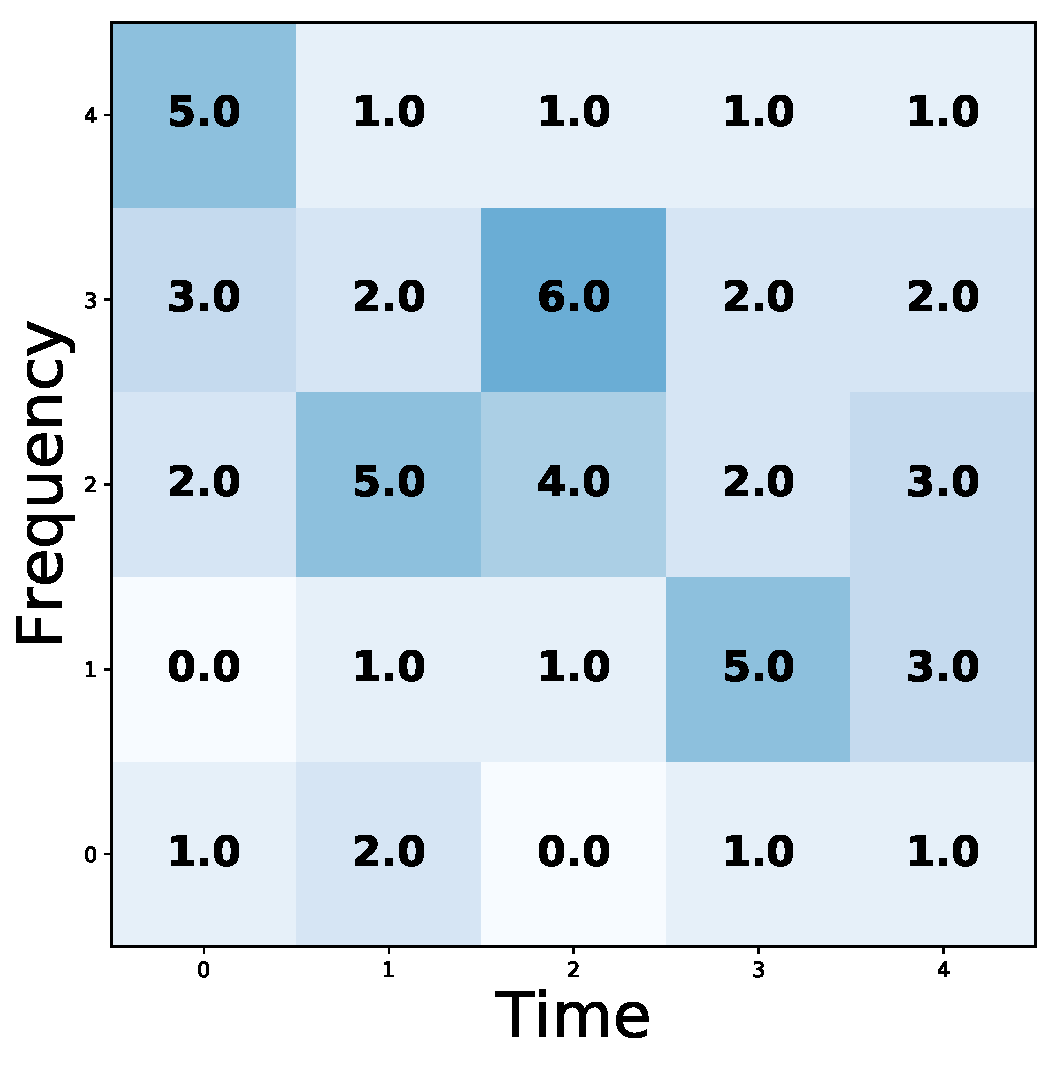
\includegraphics[width=0.8\columnwidth]{vit_data.pdf}
\caption{The input data}
\label{viterbi:plot:data}
\end{subfigure}

\begin{subfigure}[h]{0.8\columnwidth}
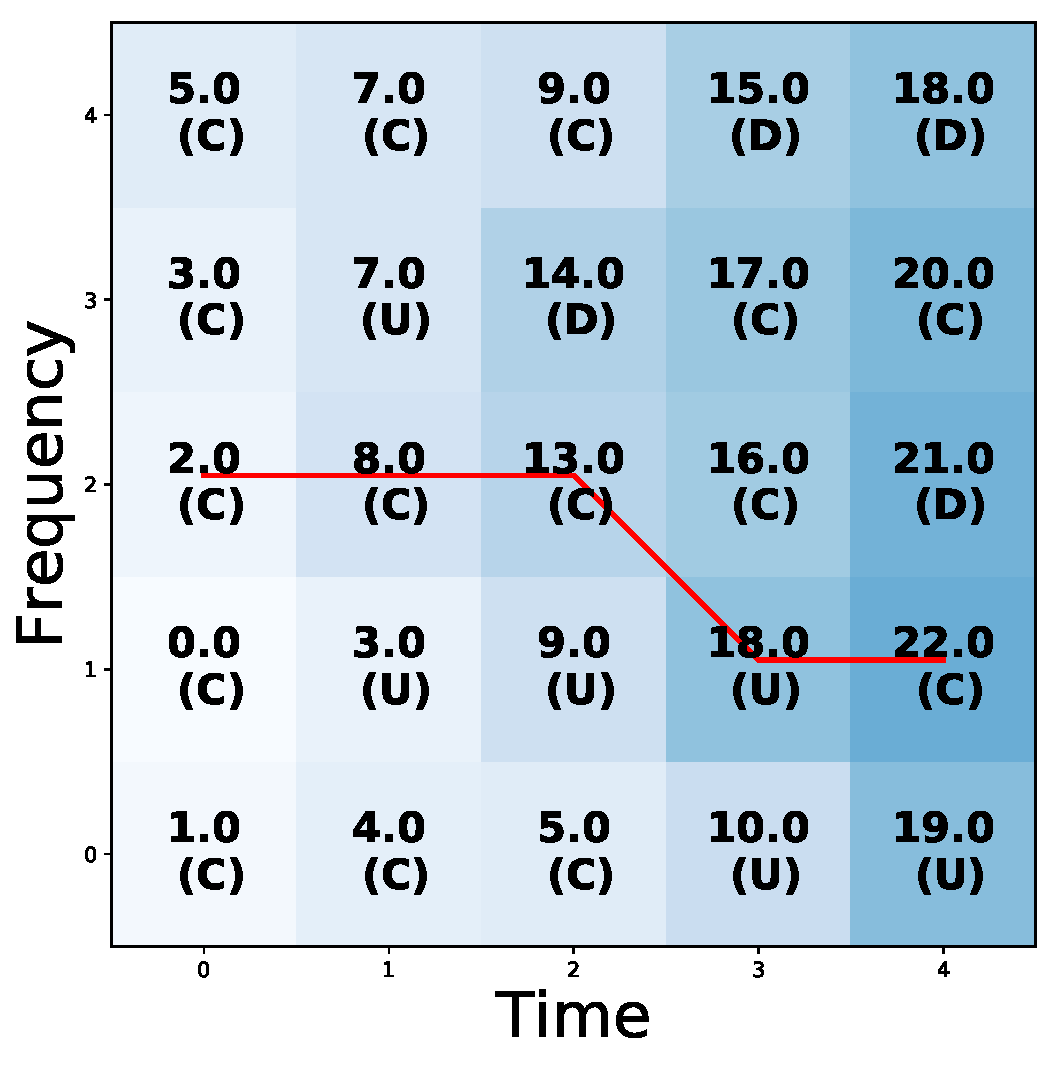
\includegraphics[width=0.8\columnwidth]{vit_prob.pdf}
\caption{The log-probabilities, jumps, and most probable path}
\label{viterbi:plot:likelihood}
\end{subfigure}

\caption{ Fig.~\ref{viterbi:plot:data} shows
the observed data, i.e the log-likelihood values $C_{j,k}$. Fig.~\ref{viterbi:plot:likelihood} shows the calculated
log-probabilities $V_{j,k}$. $A_{j,k}$ is shown in parentheses, where the \ac{UCD}
components correspond to $i= [-1,0,1]$ respectively. The red line shows the
path that gives the maximum probability. The transition matrix for the \ac{UCD} jumps is $[0,1,0]$ and corresponds to the un-normalised prior
log-probabilities of these jumps occurring.}
\label{viterbi:plots}
\end{figure}

\begin{description}
%
% Initialisation
%
\item[Initialisation] The two parts of Eq.~\ref{viterbi:maxtracklog},  $\log p(\nu_0)$ and $\log p({\bm x_0} \mid \nu_0)$, must be computed before the main recursive part of the algorithm can start. Therefore, the initialisation section (lines 5--8) in Alg.~\ref{viterbi:single:algorithm} calculates the first column in the lower panel of Fig.~\ref{viterbi:plots}. A priori, there is no preferred initial frequency, so we take the log-prior $\log p(\nu_{0,k})$ to be uniform over the complete frequency range. As a result, this is does not affect the maximisation for any jump, therefore, can be omitted from the calculation. We then use the pre-calculated log-likelihood values $C_{0,k}$ to fill the track probabilities $V_{0,k}$.  There is no previous position to jump from in this case, so the transition probabilities are irrelevant and $A_{0,k}$ are set to zero.
%
% Iteration
%
\item[Iteration] The main part of the calculation is the sum in Eq.~\ref{viterbi:maxtracklog}. Lines 11--16 in Alg.~\ref{viterbi:single:algorithm} calculate the most probable tracks that end at each frequency bin for each segment by using
    \begin{equation} \label{viterbi:single:vitsum}
    V_{j,k} = \max_{i}({C_{j,k} }+ T_{i} + V_{j-1,k+i}),
    \end{equation}
    where $i$ is the size and direction of the jump. For example, in Fig.~\ref{viterbi:plots} columns 1--4 are calculated in order using Eq.~\ref{viterbi:single:vitsum}, where it maximises over three possible previous positions in frequency. These positions are the frequency bins \ac{UCD} of the current position. The size and direction of the jump, $i$, which gives the maximum probability is then saved to $A_{j,k}$. These are shown in parentheses below the log-probabilities in Fig.~\ref{viterbi:plots} where \ac{UCD} correspond to values of $i = [-1,0,1]$ respectively.
%
% Identification
%
\item[Identification] The final stage of the algorithm identifies the most probable track. This is done by initially finding the highest log-probability values in the final time segment, $\max_k(V_{N-1,k})$ (line 19 in Alg.~\ref{viterbi:single:algorithm}). In the lower panel of Fig.~\ref{viterbi:plots} this is located at position $j,k = 4,1$ with $V_{4,1} = 22$. To find the track which corresponds to this, the values in $A_{jk}$ are followed backwards from this position (lines 20--21). For example, in Fig.~\ref{viterbi:plots} the final position is $j,k = 4,1$ and $A_{j,k} = \rm{Center} = 0$, this means that at the previous segment the most probable track was at position $j,k = 4-1,1+0 = 3,1$. At this time $A_{3,1} = R = 1$, therefore, the next track element is at $j,k = 3-1,1+1 = 2,2$. This then continues until $j=0$ whereupon these retraced positions constitute the most probable track, highlighted in red in Fig.~\ref{viterbi:plots}.
%
\end{description}

%
% mention the limitations - only returns max track.
%
The most probable track is the one traced backwards from the highest probability final segment frequency position. However, tracks can also be traced back from any of the end-frequency positions, returning the most probable track conditional on a given final position. Such tracks should not be confused with the being equal to the second, third, fourth, etc. most probable tracks. Information regarding the rankings and properties of all possible tracks (excluding the most probable and conditionally most probable tracks) is lost during the maximisation procedures computed at each stage in the algorithm --  a necessary consequence of the algorithm's speed and efficiency.

%%%%%%%%%%%%%%%%%%%%%%%%%%%%%%%%%%%%%%%%%%%%%%%%%%%%%%%%%%%%%%%%%%%%%%%%%
%%%%%%%%%%%%%%%%%%%%%%%%%%%%%%%%%%%%%%%%%%%%%%%%%%%%%%%%%%%%%%%%%%%%%%%%%
\section{\label{viterbi:multidet}Multiple detectors}
%%%%%%%%%%%%%%%%%%%%%%%%%%%%%%%%%%%%%%%%%%%%%%%%%%%%%%%%%%%%%%%%%%%%%%%%%
%
% introduce what multidetector means
%
If there are $Q$ detectors operating simultaneously we have $Q$ sets of data which can be combined appropriately to provide input to the Viterbi search described above. We must also modify the allowed transitions encoded within the transition matrix to take account of the extra prior constraints that are now available.

%
% Doppler shift at each detector
%
The received instantaneous frequency of a given astrophysical signal will be nearly the same for all ground-based \ac{GW} detectors, and our
algorithm should be sensitive to tracks that show this consistency in
frequency. However there \emph{will} be small differences between the frequencies measured at detectors that are not co-located, due to differential Doppler shifts caused by Earth rotation. As a result the signal could fall in different frequency bins at each detector.

\iffalse
To sufficient accuracy, the difference in frequency $\Delta f^{(1,2)}$ seen by two detectors ($1$ and $2$), is simply
%
\begin{equation}
\label{viterbi:multidet:doppler}
\Delta f^{(1,2)} = \frac{({{\bm v}^{(1)}} -{{\bm v}^{(2)}})\cdot{\bm \theta}}{c} f_0,
\end{equation}
%
where ${\bm v}_a$ is the velocity of detector $a$ in an inertial reference frame, $\bm \theta$ is a unit vector in the direction of the source and $f_0$ is the instantaneous signal frequency in the reference frame. The maximum difference would occur for two detectors on the equator separated by 180 degrees of longitude and for a source located in the equatorial plane, giving
%
\begin{equation}
\label{viterbi:multidet:doppler:diff}
\Delta f_{\rm max}  \approx 3.1\times 10^{-6} f_0.
\end{equation}
%
For a signal frequency of 200\,Hz the largest possible instantaneous difference in frequency between detectors is therefore $6.2\times 10^{-4}$\,Hz.  Our standard 1800\,s-long \acp{SFT} have a frequency bin-width of $5.6\times 10^{-4}$\,Hz, making this difference significant. As a result it is not enough to simply enforce that the signal tracks follow identical paths in the two detectors and we must allow some level of flexibility on the scale of $\pm 1$ frequency bin.~\chris{I find this paragraph a bit too specific to our analysis choices. We don't have to state the SFT length here. We can simply point out that you can tune the SFT length to give you differing probability distributions on your transition matrix elements. We've chosen to only 1800 sec SFTs and focus on 200\,Hz and therefore use 3 possibilities (UCD) but we could have used a different SFT length and frequency giving us any number of possible jumps. I think that we should make things easy for ourselves and state that we only ever consider 3 possibilities and then you simply tune the SFT length to your frequency spread.}
\fi

%
% Continue algorithm explanation
%
To account for these small differences in signal tracks in each detector, we reference the observed tracks to a third (pseudo) detector located at the centre of the Earth which would be insensitive to Earth spin. The signal frequencies in each real detector are then allowed to vary within a certain number of frequency bins from the track in the reference detector. In the examples that follow, we only consider the possibilities that the track in each real detector is no more that one frequency bin away from the reference track. We can tune the length of the \acp{SFT} to ensure this is a valid assumption.
As well as differences in signal frequency, due to antenna patterns and other effects, the measured signal amplitude may differ between the detectors. In the following example we assume that the signal has the same amplitude in each detector, however, in Sec.~\ref{viterbi:las} we discuss the case where they differ.

We will now show how the algorithm in Sec.~\ref{viterbi:single} can be modified to handle a two-detector network (i.e., $Q=2$),  however any number of detectors can easily be accommodated. In the two detector case the joint probability of two (real) tracks, $\nu^{(1)}$ and $\nu^{(2)}$, and the geocentric track $\nu$, given the data, is
%
\begin{equation}
\begin{split}
p(\nu,\nu^{(1)},\nu^{(2)} | D^{(1)},D^{(2)}) \propto p(\nu)p(\nu^{(1)},\nu^{(2)} | \nu) \\
p(D^{(1)} | \nu^{(1)})p(D^{(2)} | \nu^{(2)}),
\end{split}
\end{equation}
%
where $D^{(1)}$ and $D^{(2)}$ represent the data from the two detectors. The
main difference between this and that described in Sec.~\ref{viterbi:single} is
that the track probabilities $V_{j,k}$ are stored for the geocentric
pseudo-detector. The main iterative calculation (defined for the single
detector case in Eq.~\ref{viterbi:single:vitsum}) now becomes
%
\begin{equation}
\label{viterbi:multidet:vitsum}
  V_{j,k} = \max_{i,l,m}({C}^{(1)}_{j,k+l} + {C}^{(2)}_{j,k+m} + T_{i,l,m} +V_{j-1,k+i}),
\end{equation}
%
where ${C}^{(1)}$ and ${C}^{(2)}$ refer to the log-likelihoods in detectors 1 and 2 respectively and the transition matrix $T$ is an $n_1\times n_2 \times n_3$ matrix, where $n_1$ dimension refers to the jump from the previous time step, $n_2$ and $n_3$ refer to the relative frequency positions in each real detector. The transition matrix is now three-dimensional and holds the prior log-probabilities of $p(\nu)$ and $p(\nu^{(1)},\nu^{(2)} | \nu)$.  We now need to maximise over three indices: $i,l$ and $m$. The index $i$ refers to the size and direction of the jump at the geocentre (as before). The indices $l$ and $m$ refer to the number of frequency bins by which the two real tracks deviate from the geocentre track. For example, if the most probable track in the geocentred detector is in bin $j,k = 5,12$ and the values of $i,l,m = 0,-1,1$, then detector 1 is in position $j,k={5,11}$ and detector 2 is in position $j,k={5,13}$ and the geocentred track was in the position $j,k={4,12}$ at the previous time step. As a result, the track at the geocentre is only affected by Doppler modulations from the Earth's orbit whereas the tracks in the real detectors include Doppler modulations from the Earth's spin.

%
% More details on the doppler constraints
%
At every time step the frequency bin position for each real detector is forced to be within $n_l$ or $n_m$ bins of the track in the geocentred detector, where $n_l$ and $n_m$ depend on how much each detector could possibly be Doppler shifted. As mentioned previously, we only consider the case where $n_l=1$ and $n_m = 1$,  allowing the track from each real detector to be at most one frequency bin away from the geocentred track position. While we tune the \ac{SFT} length to keep this condition for different frequencies, it is also possible to tune the values of $n_l$ and $n_m$ to get a similar effect.
%
% how do we do this in practice?
%
The implementation of the multi-detector algorithm is similar to the single detector case described in Sec.~\ref{viterbi:single}.  However in the single detector case there is only a single variable to be maximised over for each time-frequency bin. This variable is the frequency jump from the position in the previous segment. For the multi-detector case there are at least three variables to be maximised over: the probability of the jump, $i$, at the geo-centre and the probability of the signal being in the surrounding positions in each on $Q$ real detectors, $l,m,\dots$. The values of $i,l,m, \dots$ are then saved to $A_{j,k}$ and are ultimately used to reconstruct the most probable consistent tracks in each real detector.

%
%  algorithm explanation
%
As in Sec.~\ref{viterbi:single}, there are three main sections: Initialisation, iteration, and the identification. For the multi-detector case each element is modified as follows.

\begin{description}
% first step calculation
\item[Initialisation] The first-row calculation (lines 5--8) in Alg.~\ref{viterbi:single:algorithm}, are now modified to additionally maximise over the real detector track positions $l$ and $m$. For each time-frequency bin the maximum sum of the log-likelihoods is saved together with the frequency locations of the corresponding tracks in the real detectors. The index $i=0$ is kept constant as there is no previous position.

% all other steps calculation
\item[Iteration] To process the subsequent time segments, lines 13--14 in Alg.~\ref{viterbi:single:algorithm} are modified to account for two (or more) detectors. Line 13 of Alg.~\ref{viterbi:single:algorithm} is changed to calculate Eq.~\ref{viterbi:multidet:vitsum}, the log-probability of a track at the geocentre ending in bin $j,k$ given that signal is in the real detector positions of $j,k+l$ and $j,k+m$. Line 14 is then modified so that $A_{j,k}$ stores the jump values, $i$, and the real detector positions, $l$ and $m$, which returned the highest probability.

% finding the most probable track
\item[Identification] The most probable track is identified in the same way as for the single detector case, first by finding the maximum value in the final time step of $V_{j,k}$ (line 19 in Alg.~\ref{viterbi:single:algorithm}). The track at the geocentre can then be found by iteratively following the jump values stored in $A_{j,k}$ back from this position. The track in each of the real detectors is determined by using the values of $l$ and $m$ indices also stored in $A_{j,k}$ to find the relative position of the track in each real detector compared to the geocentre.
%
\end{description}

This method can be extended to more than two detectors by including additional datasets and expanding the corresponding number dimensions of the maximisation procedures in the iterative steps.

%%%%%%%%%%%%%%%%%%%%%%%%%%%%%%%%%%%%%%%%%%%%%%%%%%%%%%%%%%%%%%%%%%%%%%%%%
%%%%%%%%%%%%%%%%%%%%%%%%%%%%%%%%%%%%%%%%%%%%%%%%%%%%%%%%%%%%%%%%%%%%%%%%%
\section{\label{viterbi:memory} Memory}
%%%%%%%%%%%%%%%%%%%%%%%%%%%%%%%%%%%%%%%%%%%%%%%%%%%%%%%%%%%%%%%%%%%%%%%%%
%
% general idea of memory
%
In this section we extend the basic Viterbi algorithm to improve its sensitivity to non-stochastic signals where there is some knowledge of its frequency evolution.
We do this by including a form of `memory' and this extension applies to both the single and multiple-detector cases.
Rather than considering only the previous step in our decision-making process, we now include the previous $m+1$ steps and expand the transition matrix to include these values.
A memory of $m=0$ therefore corresponds to the methods described in previous sections.
With a non-zero memory the transition matrix can a-priori make certain sequences of jumps more probable and assign different prior probabilities for these jump sequences e.g., `up then centre' may be less preferable to `centre then centre'.
As a result we can increase the chance of the most probable track matching an expected astrophysical signal.
In a single detector search with a memory of $m=1$, if we only allow \ac{UCD} transitions, then for every frequency bin we save 3 values. These are proportional to the log-probabilities of a track coming from a \ac{UCD} bin in the previous time step, where the maximisation is over the corresponding \ac{UCD} bins two time steps back.
Eq.~\ref{viterbi:multidet:vitsum} then is then modified to,
%
\begin{equation}
\label{viterbi:memory:stat}
V_{j,k,s} = \max_{h} ({C}_{j,k} + T_{s,h} +  V_{j-1,k+s,k+s+h}),
\end{equation}
%
where $s$ and $h$ refer to the \ac{UCD} jumps at the time step $j-1$ and $j-2$ respectively.  Similar to the previous two sections, the algorithm is split into three parts: initialisation, iteration, and the track identification:

\begin{description}
% initialisation
\item [Initialisation] The initialisation process needs to populate the first $m+1$ steps before the main iteration can start. At the first time step, the elements $V_{0,k,s}$ are set to the log-likelihoods $C_{0,k}$ as in Sec.~\ref{viterbi:single}.  There is no previous time step, so the element $s$ is not relevant. At the second time step, $V_{1,k,s}$ is calculated using Eq.~\ref{viterbi:memory:stat}, where there is no maximisation over $h$, it is assumed to be $0$, or a center jump. As there is no data before $j=0$, the maximisation at this point will always return the jump which has the largest prior probability, which in this case is a center jump. Therefore, the maximisation returns the same value for all frequency bins and can be set to a center jump.

%Iteration
\item [Iteration] For all following time steps the values for each element of $V_{j,k,s}$ in Eq.~\ref{viterbi:memory:stat} are calculated. This quantity is proportional to the log-probability of the track ending in time-frequency bin $j,k$, which was in the previous position of $j-1,k+s$. The corresponding value of $h$ that maximised the log-probability of the track is recorded in $A_{j,k,s}$.

%Identification
\item [Identification] The most probable track is identified in a similar way to the non-memory cases, by finding the highest-valued last element, $V_{N-1,k,s}$. The values of $s$ and $h$ are then followed back to find the most probable track. As an example, let us assume the most probable track finishes in bin $j,k,s = 10,5,0$, where the value of $m$ is $A_{10,5,0} = 1 = \rm{up}$. The previous position is then $j,k,s=10-1,5+s,m =10-1,5+0,1=9,5,1$ with a value $A_{9,5,1} = 0 = \text{Center}$, and the next track position is $j,k,s=9-1,5+1,0=8,6,0$ etc. The values of $j,k$ along this track describes most probable path.
%
\end{description}

The number of elements over which one must search increases rapidly with memory length, and has a strong impact on the computational cost of the analysis. For the single detector Viterbi approach the number of calculations made is $3 \times N \times M$ if we only allow \ac{UCD} jumps, where $N$ and $M$ are the number of time are frequency bins respectively. When memory is included this increases to $3^{m+1} \times N \times M $.

%%%%%%%%%%%%%%%%%%%%%%%%%%%%%%%%%%%%%%%%%%%%%%%%%%%%%%%%%%%%%%%%%%%%%%%%%
%%%%%%%%%%%%%%%%%%%%%%%%%%%%%%%%%%%%%%%%%%%%%%%%%%%%%%%%%%%%%%%%%%%%%%%%%
\section{\label{viterbi:sumdata}Summed input data}
%%%%%%%%%%%%%%%%%%%%%%%%%%%%%%%%%%%%%%%%%%%%%%%%%%%%%%%
%
% describe what we propose to do with summed SFT power
%
In this section a method of incoherently-summing a set of \acp{SFT} to increase the \ac{SNR} of a signal in a segment is outlined. To be more precise, it is actually the log-likelihoods which are summed, i.e. the quantity in Eq.~\ref{viterbi:periodogram}. We can write the new summed set of data $F_j$ as,
%
\begin{equation}
F_j = \sum_{i}^{N_s}C_{i,k}
\end{equation}
%
where $N_s$ is the number of \acp{SFT} to sum together and the log-likelihood $C(\nu_{i,k})$ is defined in Eq.~\ref{viterbi:periodogram}.
We can see this is possible by looking at Eq.~\ref{viterbi:single:likelihood}, where we can use the product of likelihoods,
%
\begin{equation}
\begin{split}
p(D \mid \nu) &\propto p(x_1,x_2 \ldots x_n \mid \nu) \\
&\propto p(x_1 \mid \nu) \ldots p(x_n \mid \nu) \\
&\propto \exp{\left( \sum_i C_{j,k}\right)}.
\end{split}
\end{equation}
%
If the data contains gaps where the detector was not observing, then we fill the gaps in the power spectrum with a constant value which is the expectation value of the log-likelihood. The procedure of filling in the gaps of the data is completed before any summing.  Therefore, the data should have the same mean regardless of how much real data is in each sum. In the examples that follow, we sum the \acp{SFT} over the length of one day.

The main motivation for summing the data is to increase the \ac{SNR} of a signal in the segments. The risk is that a signal can move between adjacent frequency bins during a day. To reduce this risk, we choose the frequency bin width such that it is more likely that a signal will be contained within a single frequency bin that cross a bin edge. In practise, to ensure that this is true, the segment or \ac{SFT} length and the number of segments which are summed can be tuned for each search. As well as increasing the \ac{SNR}, summing over one day should average out the antenna pattern. This means that the log-likelihood value in any bin should be more similar between detectors, however, there is still some variation due to the sky localisation and polarisation.

This also has two main effects on the transition matrix, the first is that as each segment of data is now one day long, a jump between frequency bins is far more likely, therefore, the transition matrix elements are modified to account for this. The second is that as the data is averaged over one day, the signal should remain is the same frequency bin between detectors, therefore, there is no longer a need for the multi-dimensional transition matrix described in Sec.~\ref{viterbi:multidet}.

The volume of the data is also reduced by a factor of $1/N_s$, therefore, the time taken for the algorithm to run is also reduced by the same factor.

%%%%
% EXTRA INFO NOT INCULDED AT THE MOMENT
%%%%%%%
\iffalse

Using the same example in Sec.~\ref{viterbi:multidet}, we have two detectors that are at opposite sides of the earth on the equator.
A signal in the equatorial plane at 150\,Hz will have a spread of frequency of $\Delta f = 3.1 \times 10^{-6} \times 150 \; \rm{Hz} = 4.7 \times 10^{-4} \; \rm{Hz}$.
This is less than the bin width of our 1800\,s \acp{SFT} which is $5.6 \times 10^{-4} \; \rm{Hz}$.
Therefore, over the course of one day the signal should spend most of its time within one \ac{SFT} frequency bin.
For the real \ac{LIGO} detectors this will be less due to their locations, therefore, we can assume that the signal stays within one frequency bin for the duration of a day.
This then allows us to sum the \acp{SFT} over one day, i.e. as we have 1800\,s long \acp{SFT}, we can add every 48 together.

\fi
%%%%%%%

%%%%%%%%%%%%%%%%%%%%%%%%%%%%%%%%%%%%%%%%%%%%%%%%%%%%%%%%%%%%%%%%%%%%%%%%%
%%%%%%%%%%%%%%%%%%%%%%%%%%%%%%%%%%%%%%%%%%%%%%%%%%%%%%%%%%%%%%%%%%%%%%%%%
\section{\label{viterbi:las}Line-aware statistic}
%%%%%%%%%%%%%%%%%%%%%%%%%%%%%%%%%%%%%%%%%%%%%%%%%%%%%%%%%%%%%%%%%%%%%%%%%
%
% what is the line aware statistic
%
The multiple-detector algorithm described in Sec.~\ref{viterbi:multidet} returns the most probable track of a common signal assumed to be in Gaussian noise. As a consequence the algorithm will return large values of the log-likelihood even if there are inconsistent values of \ac{SFT} power between the detectors, either from non-Gaussian noise or because the signal is not equally strong in the two detectors. However a signal with unequal power in the two detectors is more likely to be a non-Gaussian instrumental line than an astrophysical signal. The line-aware statistic described in this section is designed to make the search more robust to such instrumental artefacts within realistic non-Gaussian data whilst maintaining sensitivity to astrophysical signals.

%
% More detail on what this is applied to
%
For most of the analysis examples presented here we use data which is the incoherent sum of 30-minute normalised \acp{SFT} over a day (described in more detail in Sec.~\ref{viterbi:sumdata}). As a result the effects of the detector antenna patterns and of differential Doppler shifts are significantly reduced, and any signal should have a broadly similar summed log-likelihood in the same frequency bin in each detector. The statistic can then be modified such that we expect a similar log-likelihood in each detector.

We first consider the model of Gaussian noise with no signal present. Within
a single summed segment, the likelihood of Gaussian noise at
frequency $\nu$ is given by a $\chi^2$ distribution,
%
\begin{equation}
\label{las:central}
p(F_j|\nu_j,M_{\text{N}},I) = \frac{1}{2^{d/2}\Gamma(d/2)}F_j^{d/2 - 1}\exp{\left\{
\frac{F_j}{2}\right\}}
\end{equation}
%
where $F_j$ is the frequency domain power summed over sub-segments within a single day, as described in Sec.~\ref{viterbi:sumdata} and  $d$ is the number of degrees of freedom,  equal to twice the total number of summed SFTs.  $M_{\rm{N}}$ represents the model that the data is simply Gaussian noise. In the presence of a signal (model $M_{\text{S}}$), the power should follow a non central $ \chi^2 $ distribution in which the non-centrality parameter $\lambda$ is the square of the \ac{SNR}, $(\lambda = \rho_{\rm{opt}}^2 )$, i.e.
%
\begin{equation}
\label{las:noncentral}
\begin{split}
p(F_j|\nu_j,\lambda,M_{\text{S}},I) = \frac{1}{2} \exp{\left\{ -\frac{F_j+\lambda}{2}\right\}} \left( \frac{F_j}{\lambda} \right)^{d/4 - 1/2} \\
I_{d/2 -1}\left( \sqrt{\lambda F_j}\right).
\end{split}
\end{equation}
%
If a signal is present we therefore expect the \ac{SFT} powers in both detectors to follow Eq.~\ref{las:noncentral}.  Assuming for the moment that the noise variance is the same in both, we can determine the evidence for model $M_{\text{S}}$ by marginalising over $\lambda$,
%
\begin{equation}
\label{las:signal}
\begin{split}
p(F^{(1)}_{j},F^{(2)}_{j} \mid \nu_j,M_{\rm{S}},I) = \int_0^{\infty}  p(\lambda,w_{\rm_S}) \\
p(F^{(1)}_{j}|\nu_j,\lambda,M_{\text{S}},I)p(F^{(2)}_{j}|\nu_j,\lambda,M_{\text{S}},I) d\lambda.
\end{split}
\end{equation}
%
We set the prior on $\lambda$ to be an exponential distribution of width $w$, this is done somewhat arbitrarily as we expect the majority of signals to have a low \ac{SNR}. This distribution follows,
\begin{equation}
\label{las:prior}
p(\lambda,w) = \exp\left( \frac{-\lambda}{w}\right).
\end{equation}

On the other hand, if an instrumental line is present in one of the detectors we expect to see signal-like power in that detector and noise-like power in the other.  The evidence for this `line' model ($M_{\text{L}}$) is therefore
%
\begin{equation}
\label{las:line}
\begin{split}
p(F^{(1)}_{j},F^{(2)}_{j} \mid \nu_j,M_{\rm{L}},I) = \int_0^{\infty}  p(\lambda,w_{\rm_L}) \\
\left[ p(F^{(1)}_{j}|\nu_j,M_{\rm{N}},I)p(F^{(2)}_{j}|\nu_j,\lambda,M_{\rm{S}},I) \right. \\
\left. + p(F^{(1)}_{j}|\nu_j,\lambda,M_{\rm{S}},I)p(F^{(2)}_{j}|\nu_j,M_{\rm{N}},I)\right]d\lambda ,
\end{split}
\end{equation}
%
The third option to consider is the simple case of approximately Gaussian noise in both of the detectors,
%
\begin{equation}
\label{las:noise}
\begin{split}
p(F^{(1)}_{j},F^{(2)}_{j} \mid \nu_j,\lambda,M_{\rm{G}},I) = p(F^{(1)}_{j} \mid \nu_j,M_{\rm{G}},I) \\
p(F^{(2)}_{j} \mid \nu_j,M_{\rm{G}},I) .
\end{split}
\end{equation}
The posterior probability of model $M_{\text{GL}}$, which contains the probability of Gaussian noise or Gaussian noise with a line in one detector, (taken as mutually exclusive) is
\begin{equation}
\begin{split}
p(M_{\rm{GL}} \mid F^{(1)}_{j},F^{(2)}_{j},\nu_j ,I) = p(M_{\rm{G}} \mid F^{(1)}_{j},F^{(2)}_{j},\nu_j ,I) \\
+p(M_{\rm{L}} \mid F^{(1)}_{j},F^{(2)}_{j} ,\nu_j, I),
\end{split}
\end{equation}
where we assume that $M_{\rm{G}}$ and $M_{\rm{L}}$ are mutually exclusive.

%
We can now find the posterior odds ratio for the presence of a signal over noise or a line,
\begin{equation}
\label{viterbi:odds}
\begin{split}
O_{\rm{SGL}}(F^{(1)}_{j},F^{(2)}_{j}\mid\nu_j) &=  \frac{p(M_{\rm{S}} \mid F^{(1)}_{j},F^{(2)}_{j} ,\nu_j)}{p(M_{\rm{GL}} \mid F^{(1)}_{j},F^{(2)}_{j},\nu_j)}
= \frac{p(M_{\rm{S}} \mid F^{(1)}_{j},F^{(2)}_{j} ,\nu_j)}{p(M_{\rm{G}} \mid F^{(1)}_{j},F^{(2)}_{j} ,\nu_j) +p(M_{\rm{L}} \mid F^{(1)}_{j},F^{(2)}_{j} ,\nu_j)}\\
&=\frac{p(M_{\rm{S}})p(F^{(1)}_{j},F^{(2)}_{j} \mid M_{\rm{S}},\nu_j)}{p(M_{\rm{G}})p(F^{(1)}_{j},F^{(2)}_{j}\mid M_{\rm{G}},\nu_j) + p(M_{\rm{L}})p(F^{(1)}_{j},F^{(2)}_{j}\mid M_{\rm{L}},\nu_j) } \\
&= \frac{p(F^{(1)}_{j},F^{(2)}_{j} \mid M_{\rm{S}},\nu_j)p(M_{\rm{S}})/p(M_{\rm{G}})}{p(F^{(1)}_{j},F^{(2)}_{j}\mid M_{\rm{G}},\nu_j) + p(F^{(1)}_{j},F^{(2)}_{j}\mid M_{\rm{L}},\nu_j)p(M_{\rm{L}})/p(M_{\rm{N}}) }
\end{split}
\end{equation}
In practice it is convenient to use the log odds ratio,
\begin{equation}
\begin{split}
\label{viterbi:las:logodds}
\log\left[ O_{\rm{SGL}}(F^{(1)}_{j},F^{(2)}_{j})\right] &=  \log\left[ p(F^{(1)}_{j},F^{(2)}_{j} \mid M_{\rm{S}}) \right] \\
&- \left[ \log\left( p(F^{(1)}_{j},F^{(2)}_{j}\mid M_{\rm{G}}) \right. \right. \\
&\left.\left.+  p(F^{(1)}_{j},F^{(2)}_{j}\mid M_{\rm{L}})p(M_{\rm{L}})/p(M_{\rm{G}})\right) \right]
\end{split}
\end{equation}
As we are only interested in the maximum of $\log\left[ O_{\rm{SGL}}(F^{(1)}_{j},F^{(2)}_{j})\right]$, the factor $\log\left[ p(M_{\rm{S}})/p(M_{\rm{G}})\right]$ can be dropped from the expression.


In this version of the Viterbi algorithm, rather than storing a value proportional to the log-probabilities as in Sec.~\ref{viterbi:multidet}, here we store a value proportional to the log-odds ratio.
Here we take the log-odds ratio defined in Eq.~\ref{viterbi:las:logodds}, which is the log-odds of a signal having a similar power in each detector, and add the log-prior odds $p(\bm{\nu} \mid M_S)/(p(\bm{\nu} \mid M_N) + p(\bm{\nu} \mid M_L))$ which is the log-prior or any particular track. By assuming that the track transitions for the line and noise model are equally probable for any jump, we set the denominator of the prior-odds is a constant $b$.
This then means Eq.~\ref{viterbi:multidet:vitsum} is modified to,
\begin{equation}
\begin{split}
\label{lineaware:stat}
\hat{V}_{i,j} = \max_{k,l,m}\left(T_{k,l,m} + b + V_{i-1,j+k}   \right. \\
 + \left.  \log\left[O_{\rm{SGL}}\left(F^{(1)}_{j},F^{(2)}_{j}\right)\right]\right),
\end{split}
\end{equation}
%
where $\hat{V}$ refers to a log-odds ratio.
The maximised statistic now has three tuneable parameters: the width, $w_S$ in Eq.~\ref{las:prior}, on the prior for a signal \ac{SNR} squared, $p_{\rm S}(\lambda)$, the width, $w_L$ of the prior in the case of a line, $p_{\rm L}(\lambda)$, and the ratio of the prior on the line and noise models, $p({M_{\rm L}})/p({M_{\rm G}})$.  These parameters are optimised for each search, where we initially estimate the \ac{SNR} of a signal we hope to be sensitive to in each time slice, then use this as a guide for the width of the signal prior. This is then repeated for an expected line \ac{SNR} and this is used for the width of the line prior. The ratio of line and noise models runs in the range 0 to 1, we set this limit as we do not expect an instrumental line to be as likely as Gaussian noise in any particular frequency bin.

The values in Eq.~\ref{viterbi:las:logodds} can be calculated prior to the run for a range of \ac{SFT} powers. Given that 48 \acp{SFT} are summed over one day for the majority of the analysis, the normalised powers will have a mean of 96. 
Therefore, Fig.~\ref{viterbi:las:osgl_plots} shows the output of Eq.~\ref{viterbi:las:logodds} for a range of \ac{SFT} powers in each detector for 3 examples of input parameters. 
In Fig.~\ref{viterbi:lineaware:example} an example of how the `line aware' statistic improves the robustness of the algorithm against non astrophysical signals. 

\begin{figure}
    \centering
    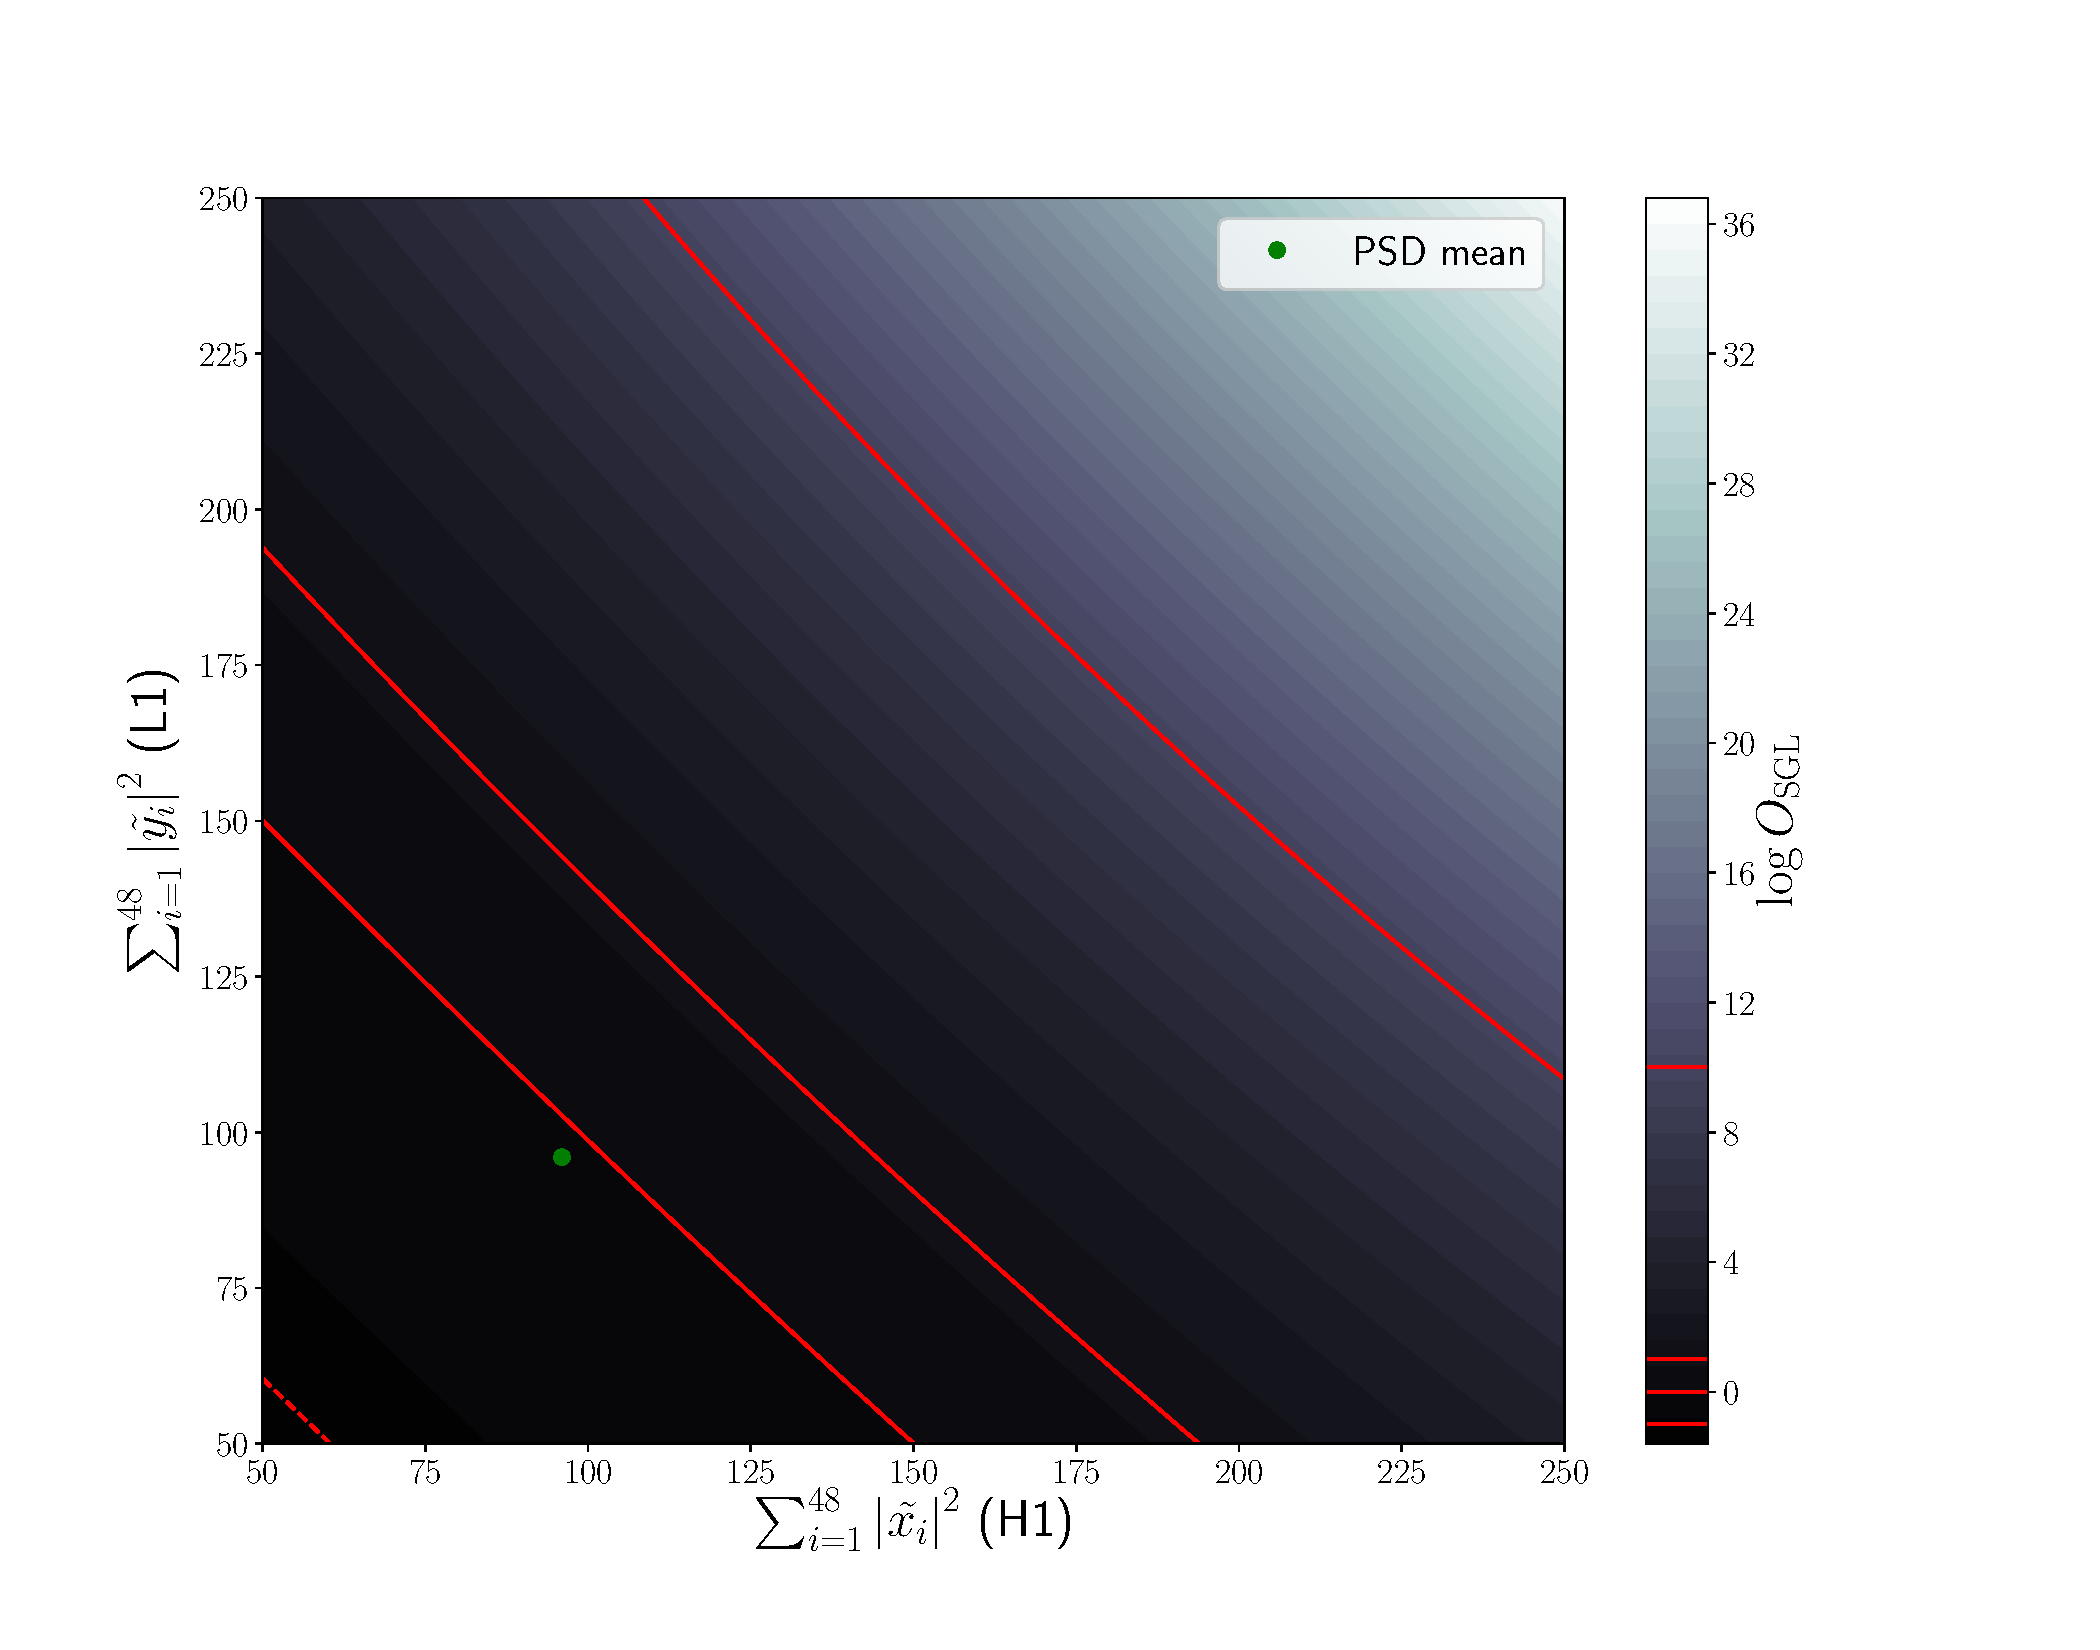
\includegraphics[width=\linewidth]{lookup_noline.pdf}
    \caption{This figure shows an example of when the line aware statistic is used compared to a version when it is not.}
    \label{fig:my_label}
\end{figure}

\begin{figure}[h]
\centering

\begin{subfigure}[h]{\linewidth}
\begin{minipage}{0.65\linewidth}
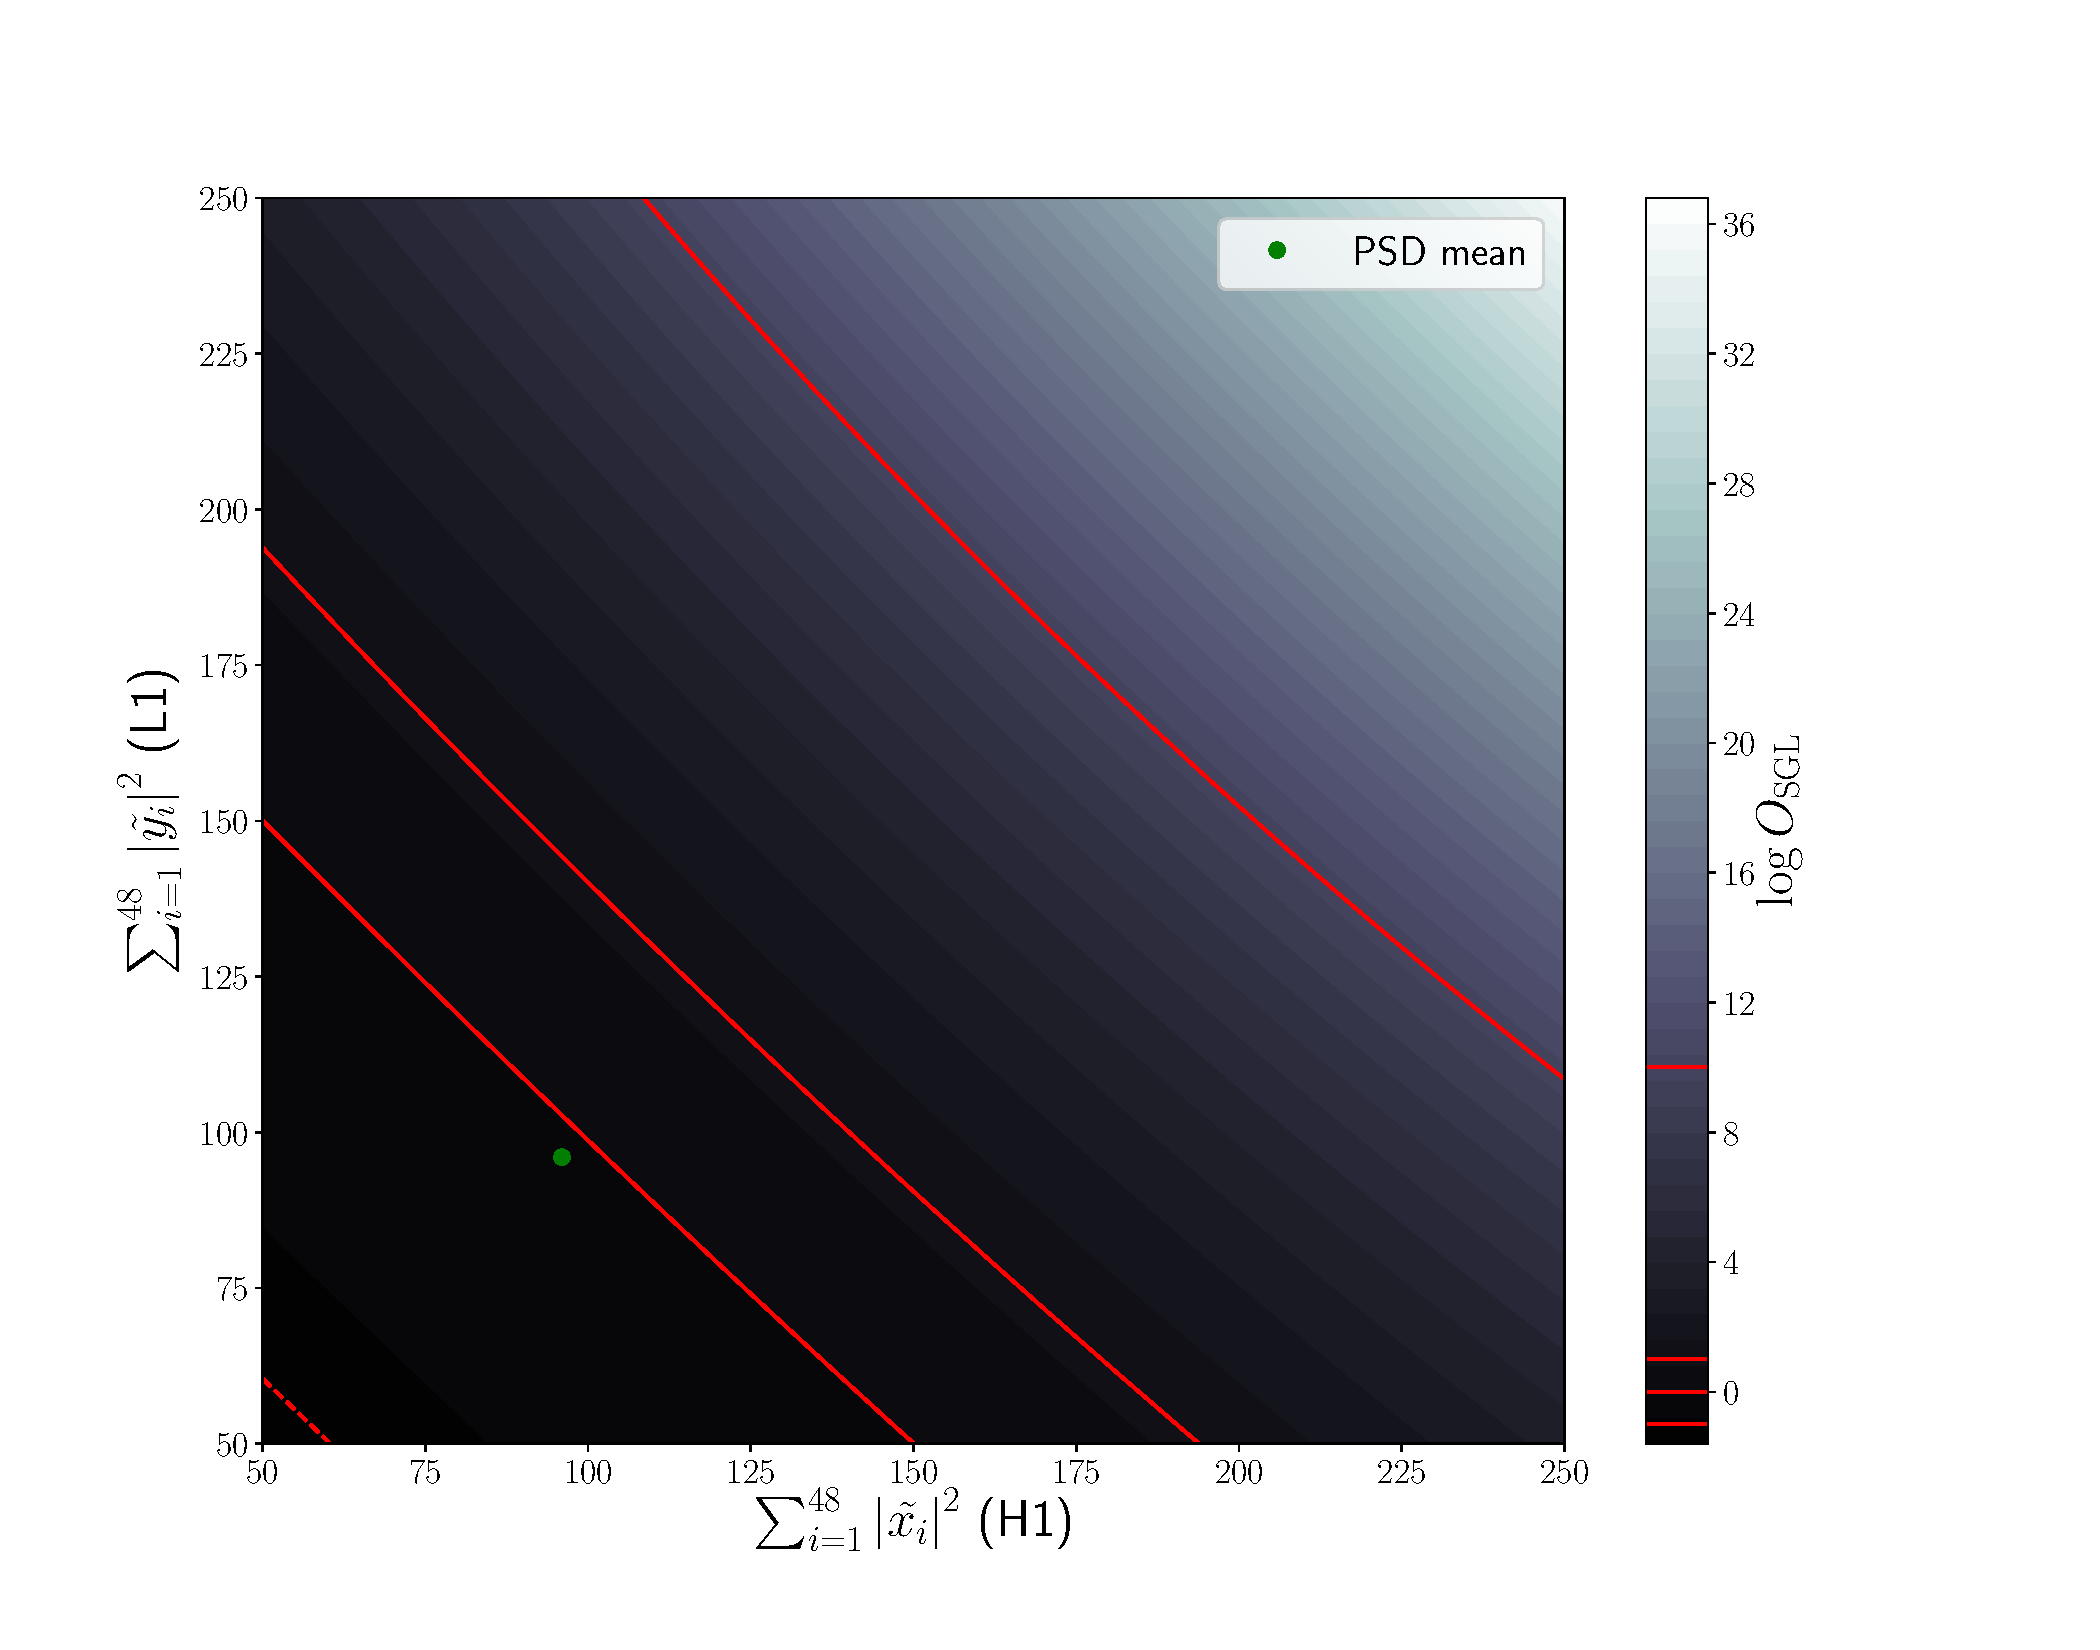
\includegraphics[width=1.\linewidth]{lookup_noline.pdf}
\end{minipage}\hfill
\begin{minipage}{0.35\linewidth}
\caption{This shows the distribution of the lines aware statistic plotted against the \ac{FFT} power in each detector. This example is for parameters $p_s(\lambda) = 2$,$p_l(\lambda) = 0$ and $p(M_L)/p(M_G) = 0$. So the line part of the statistic is not operating.}
\label{viterbi:plot:data}
\end{minipage}
\end{subfigure}

\begin{subfigure}[h]{\linewidth}
\begin{minipage}{0.65\linewidth}
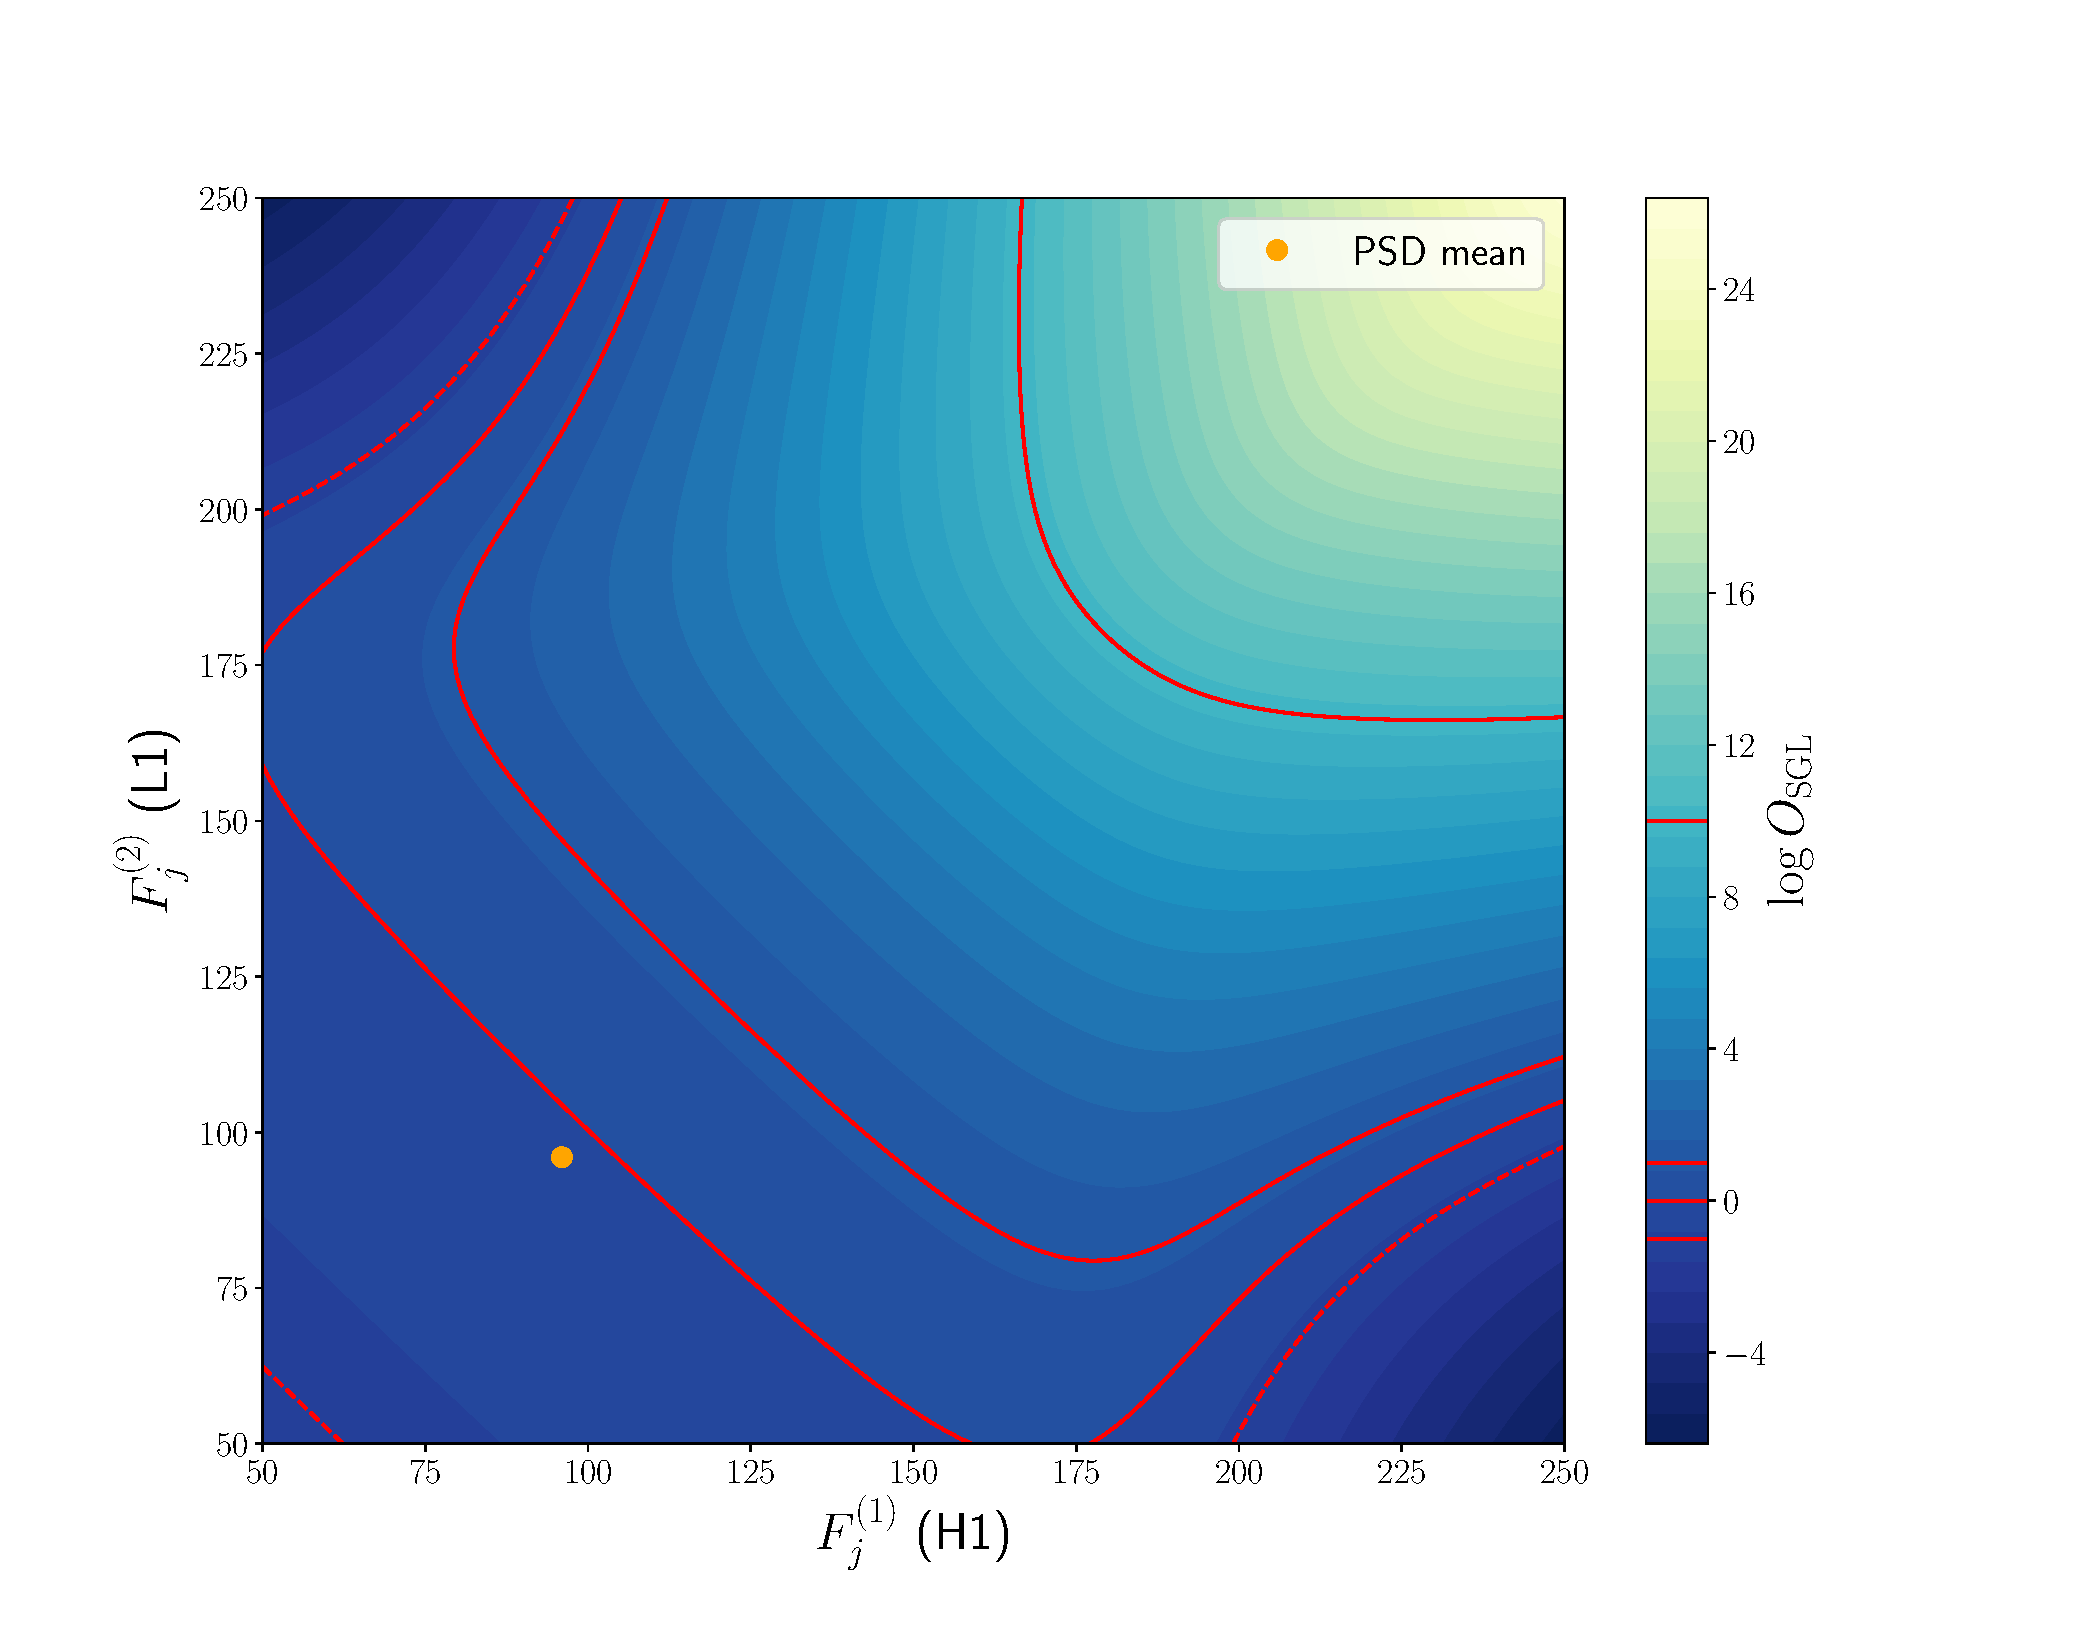
\includegraphics[width=1.\columnwidth]{lookup_linesmall.pdf}
\end{minipage}\hfill
\begin{minipage}{0.35\linewidth}
\caption{This shows the distribution of the lines aware statistic plotted against the \ac{FFT} power in each detector. This example is for parameters $p_s(\lambda) = 2$,$p_l(\lambda) = 2$ and $p(M_L)/p(M_G) = 1$. Here the line part of the statistic has the same \ac{SNR} and the signal part, i.e. we expect the \ac{SNR} of a signal to be similar to that of a line.}
\label{viterbi:plot:data}
\end{minipage}
\end{subfigure}

\begin{subfigure}[h]{\linewidth}
\begin{minipage}{0.65\linewidth}
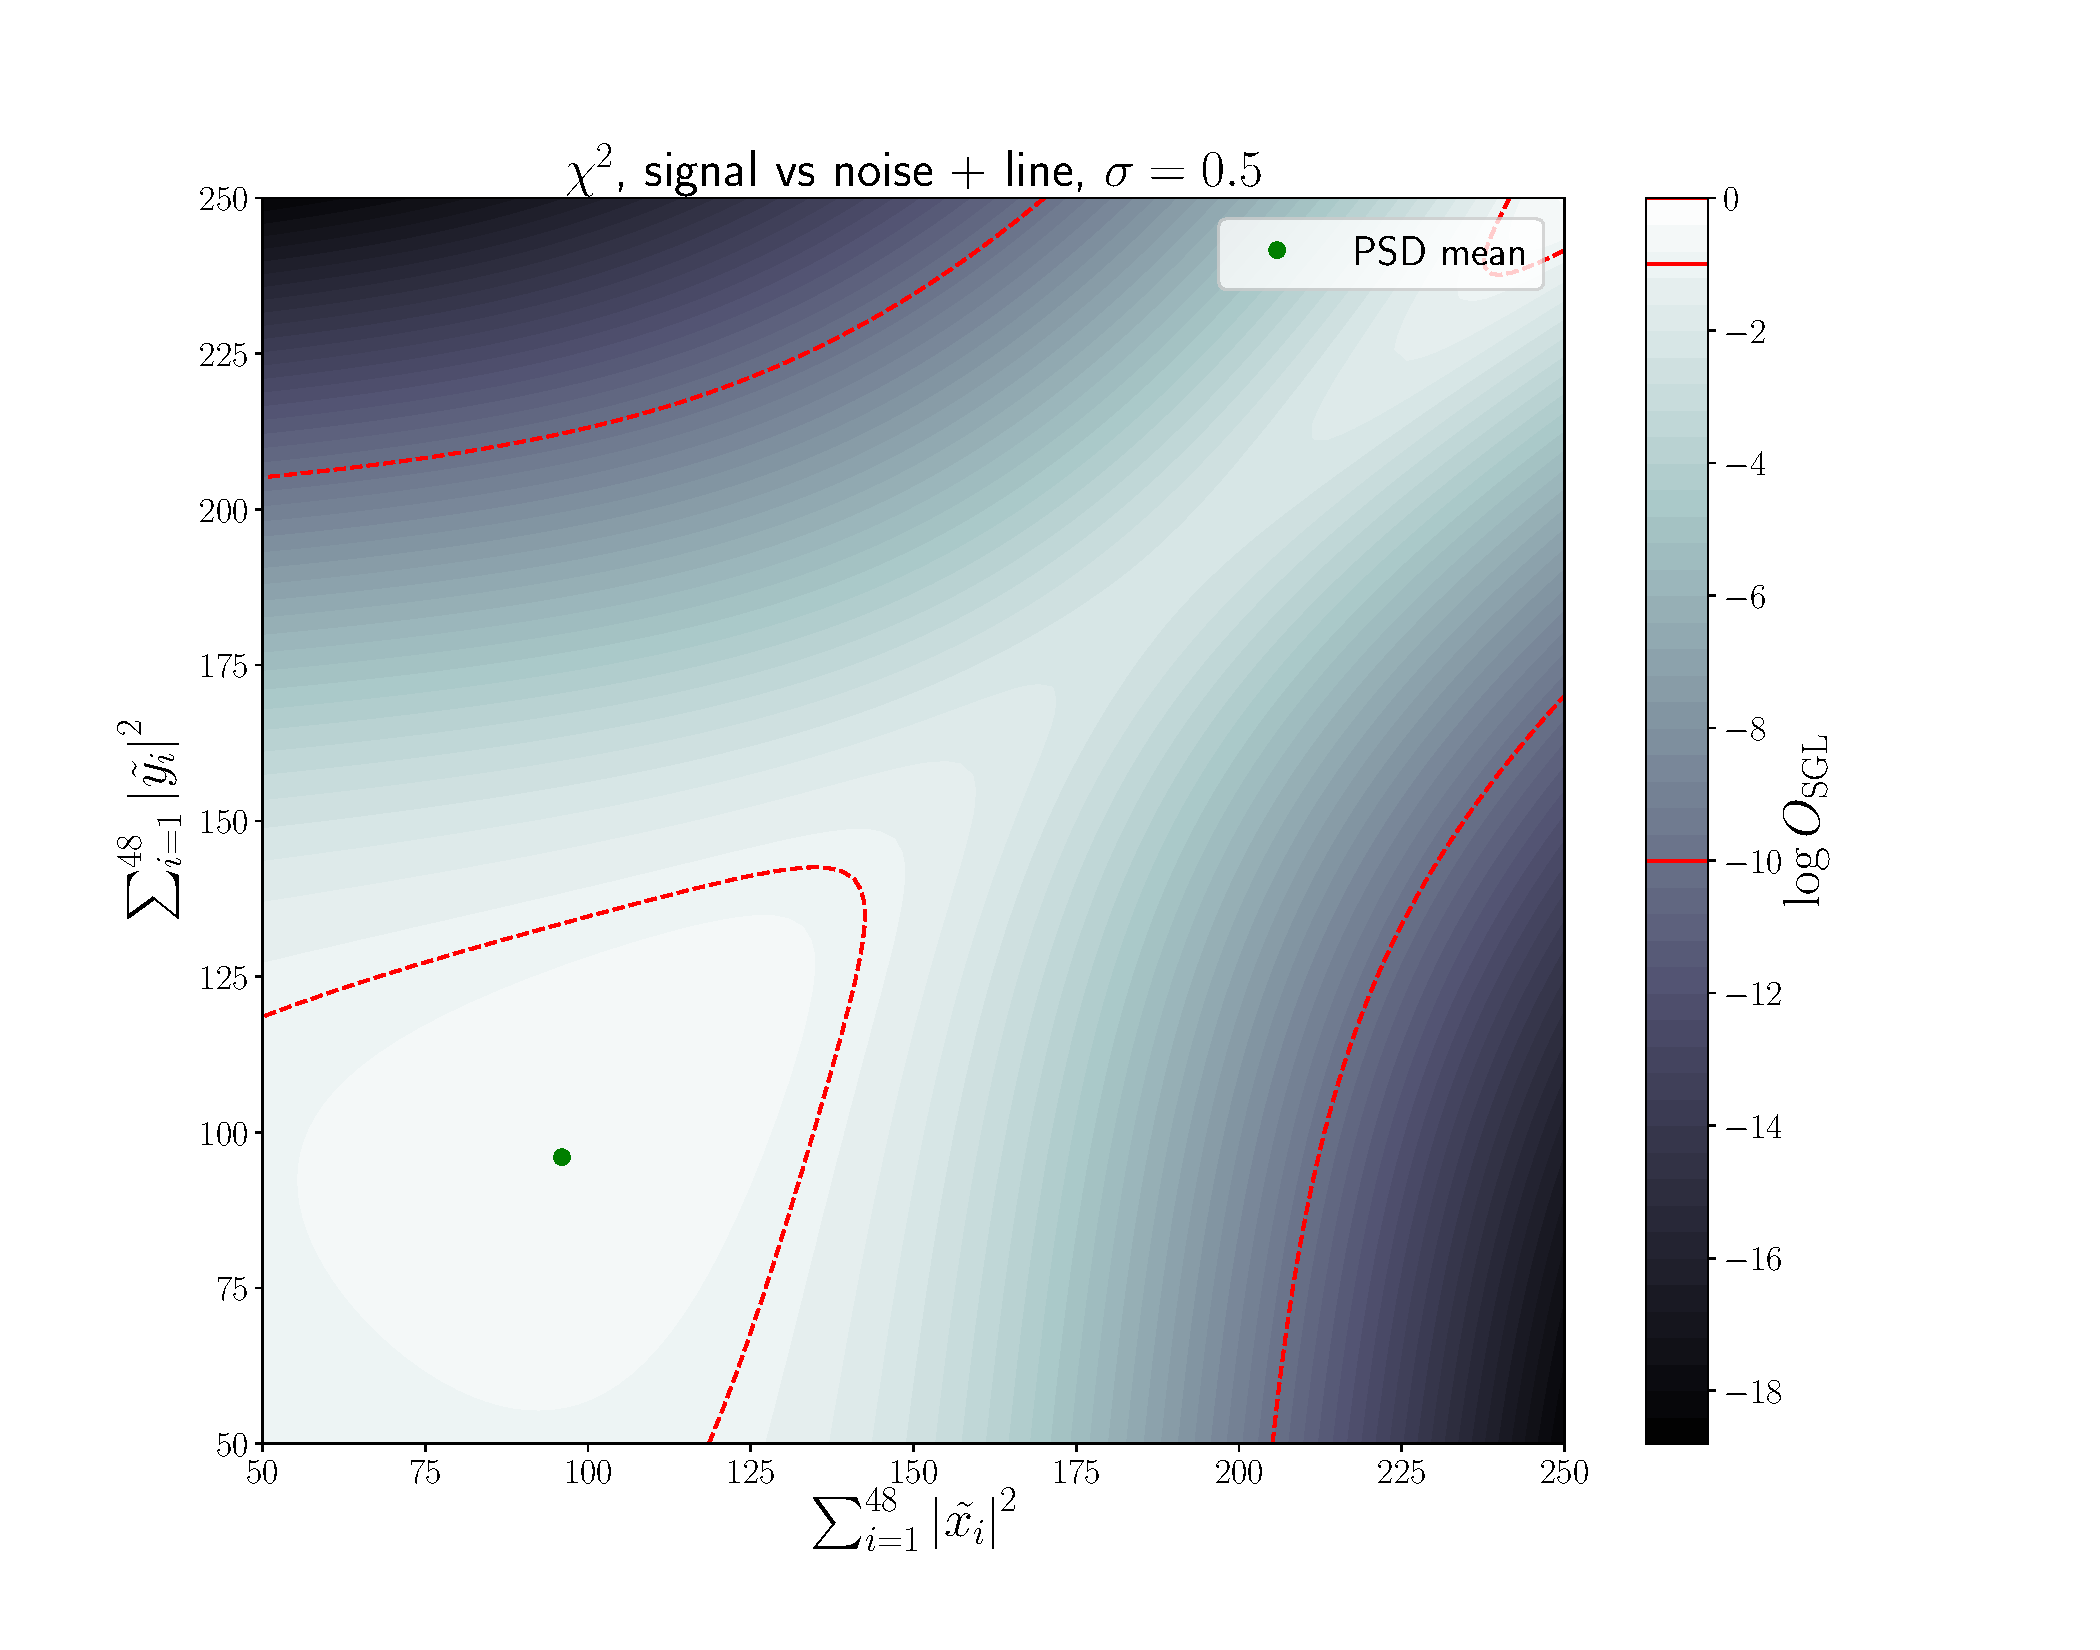
\includegraphics[width=1.\columnwidth]{lookup_linebig.pdf}
\end{minipage}\hfill
\begin{minipage}{0.35\linewidth}
\caption{This shows the distribution of the lines aware statistic plotted against the \ac{FFT} power in each detector. This example is for parameters $p_s(\lambda) = 2$,$p_l(\lambda) = 10$ and $p(M_L)/p(M_G) = 1$. Here we expect the \ac{SNR} of a line to be larger than a signal.}
\label{viterbi:plot:data}
\end{minipage}
\end{subfigure}
\caption{Lookup tables using the line aware statistic in Eq.~\ref{viterbi:las:logodds}.}
\label{viterbi:las:osgl_plots}
\end{figure}


%%%%%%%%%%%%%%%%%%%%%%%%%%%%%
%%%%%%%%%%%%%%%%%%%%%%%%%%%%%
\section{\label{viterbi:lineaware}Line aware statistic for consistent amplitude}
%%%%%%%%%%%%%%%%%%%%%%%%%%%%%
%%%%%%%%%%%%%%%%%%%%%%%%%%%%%


Above the `line aware' statistic was designed to penalise high \ac{SFT} powers in a single detector and reward powers which have a similar \ac{SNR}. This is often a useful statistic to use when the detectors have similar sensitivities, however, this is not always the case. During an observing run of a gravitational wave detector, their sensitivity will vary with time due fluctuating or new noise sources or potentially upgrades which can increase the sensitivity. A change in the sensitivity, or noise floor, affects the \ac{SNR} of a possible signal in in the data, i.e. a lower noise floor results in a higher \ac{SNR}. 
In this section the above `line aware' statistic is modified to account for the difference in sensitivities of the detectors, and therefore search for a consistent amplitude between detectors as opposed to \ac{SNR}.

There are two main factors which are taken into account when determining how sensitive a detector is in a particular time interval: the \ac{PSD} of detector and the duty cycle. A decrease in the duty cycle and an increase in the \ac{PSD} will decrease the \ac{SNR}. To search for consistent amplitude Eq.\ref{lineaware:stat} is modified by weighting each detector by its \ac{PSD} and duty cycle.

The definition of \ac{SNR} is taken from \cite{} as, 
\begin{equation}
    \rho_0^2 = \frac{h_0^2 T}{S}(\alpha_1A + \alpha_2B + \alpha_3C),
\end{equation}
where $\rho_0$ is the \ac{SNR}, $h_0$ is the signal amplitude, $T$ is the time of observation, $S$ is the noise \ac{PSD} and the term in brackets include the antenna pattern of the detector. 
The signal with amplitude $h_0$ will be the same amplitude at both detectors (H and L), therefore we can relate the \ac{SNR} in each detector by,
\begin{equation}
\label{lineawareamp:snrequate}
    \rho_L^2 = \frac{\rho_H^2 S_H T_L}{S_L T_L} \frac{(\alpha_1A_L + \alpha_2B_L + \alpha_3C_L)}{(\alpha_1A_H + \alpha_2B_H + \alpha_3C_H)} .
\end{equation}

For the majority of the analysis that follows the \acp{SFT} are summed over one day, this will be explained in greater detail in Sec.~\ref{}. The components in the above equation which have the form $(\alpha_1A + \alpha_2B + \alpha_3C)$, account for the antenna pattern of the earth as it rotates. These can be approximated to be the same for the two detectors H1 and L1, therefore we can simplify the above Eq.~\ref{lineawareamp:snrequate} to, 
\begin{equation}
\label{lineawareamp:snrratio}
    \rho_L^2 = \frac{\rho_H^2 S_H T_L}{S_L T_L} = l \rho_H^2 .
\end{equation}
This then gives a factor which relates the \ac{SNR} of each detector, where $S$ and $T$ are values that are known for a given data-set prior to running the search.

This ratio of \acp{SNR} can be included in the integral over \ac{SNR} for the signal model in Eq.~\ref{las:signal} as follows,
\begin{equation}
\label{lineawareamp:signal}
p(F^{(1)}_{j},F^{(2)}_{j} \mid \nu_j,M_{\rm{S}},I) = \int_0^{\infty}  p(\lambda,w_{\rm_S}) 
p(F^{(1)}_{j}|\nu_j,\lambda,M_{\text{S}},I)p(F^{(2)}_{j}|\nu_j,l\lambda,M_{\text{S}},I) d\lambda.
\end{equation}

Similarly the line model in Eq.~\ref{las:line} can be modified as,

\begin{equation}
\label{lineawareamp:line}
\begin{split}
p(F^{(1)}_{j},F^{(2)}_{j} \mid \nu_j,M_{\rm{L}},I) = \int_0^{\infty}  p(\lambda,w_{\rm_L}) 
\left[ p(F^{(1)}_{j}|\nu_j,M_{\rm{N}},I)p(F^{(2)}_{j}|\nu_j,l\lambda,M_{\rm{S}},I) \right. \\
\left. + p(F^{(1)}_{j}|\nu_j,\lambda,M_{\rm{S}},I)p(F^{(2)}_{j}|\nu_j,M_{\rm{N}},I)\right]d\lambda .
\end{split}
\end{equation}

Fig.~\ref{viterbi:lineawareamp:power} shows an example of the values of the statistic described in Eq.~\ref{lineawareamp:line} plotted against a range of \ac{FFT} powers from each detector. This demonstrated how the statistic accounts for a difference in sensitivity on detectors by allowing the \ac{FFT} power or effectively \ac{SNR} to vary more.

In Fig.~\ref{viterbi:lineawareamp:example} we show an example of two detectors with large differences in sensitivity, and how the statistic which takes this into account can improve the search sensitivity in this case.

\begin{figure}[h]
\centering

\begin{subfigure}[h]{\linewidth}
\begin{minipage}{0.65\linewidth}
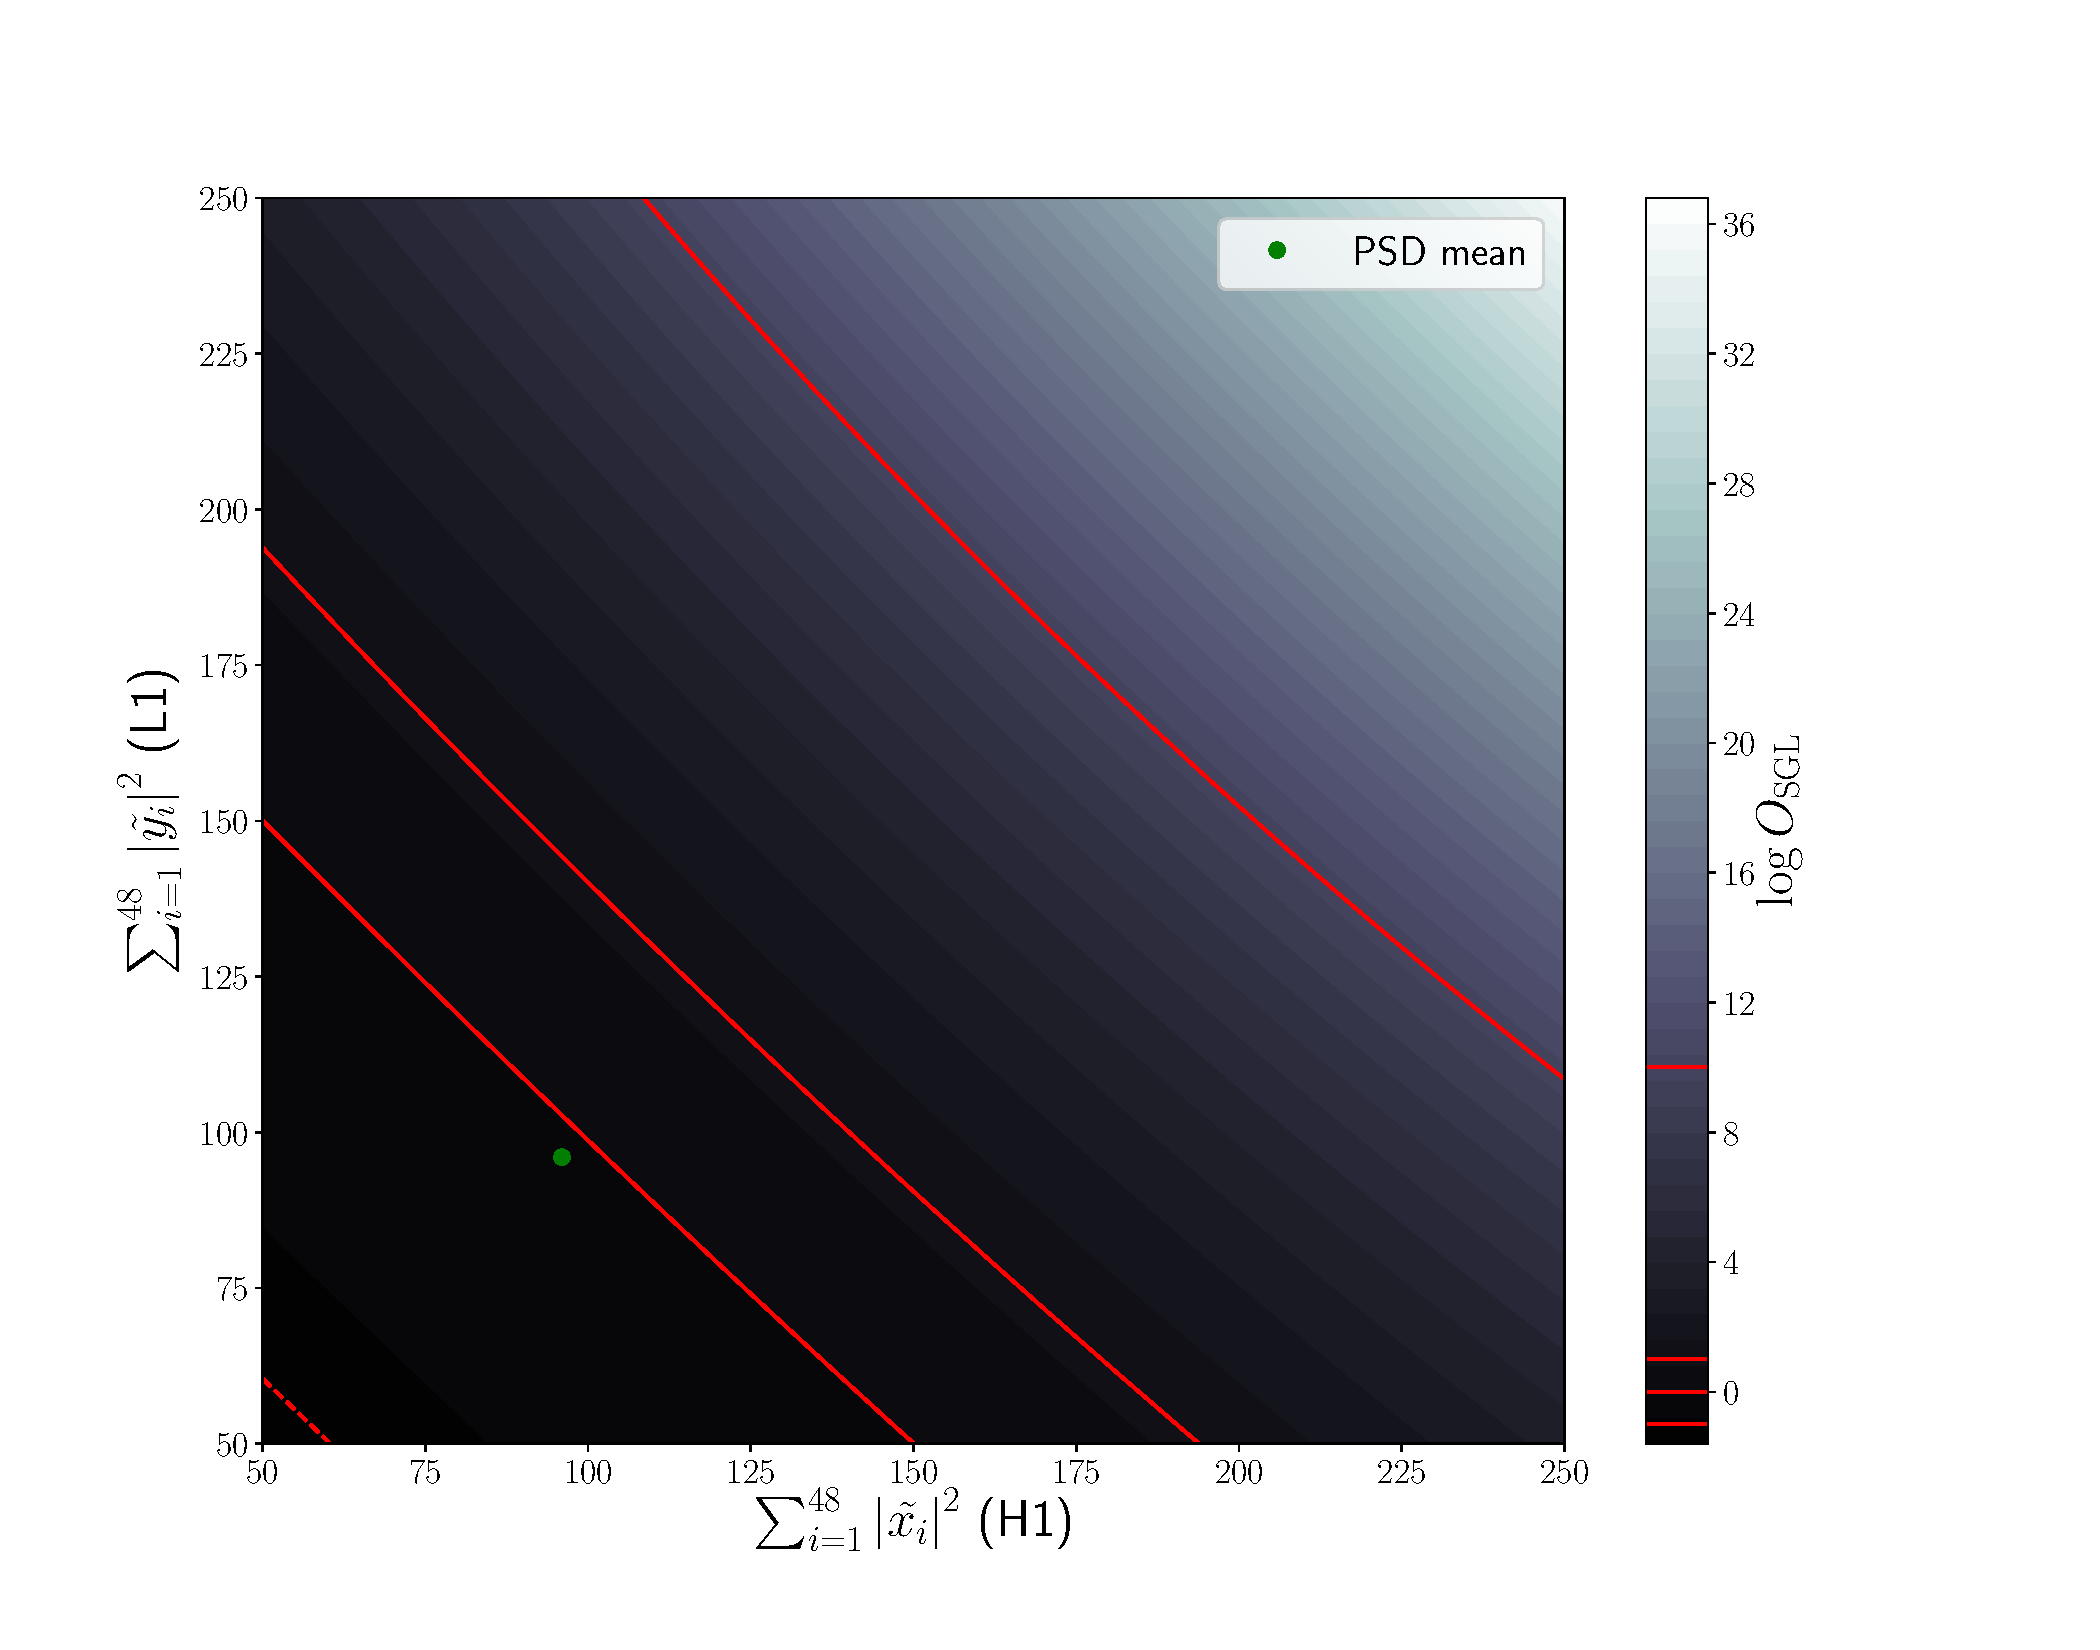
\includegraphics[width=1.\linewidth]{lookup_noline.pdf}
\end{minipage}\hfill
\begin{minipage}{0.35\linewidth}
\caption{This shows the distribution of the lines aware statistic plotted against the \ac{FFT} power in each detector. This example is for parameters $p_s(\lambda) = 2$,$p_l(\lambda) = 0$ and $p(M_L)/p(M_G) = 0$. So the line part of the statistic is not operating.}
\label{viterbi:plot:data}
\end{minipage}
\end{subfigure}

\begin{subfigure}[h]{\linewidth}
\begin{minipage}{0.65\linewidth}
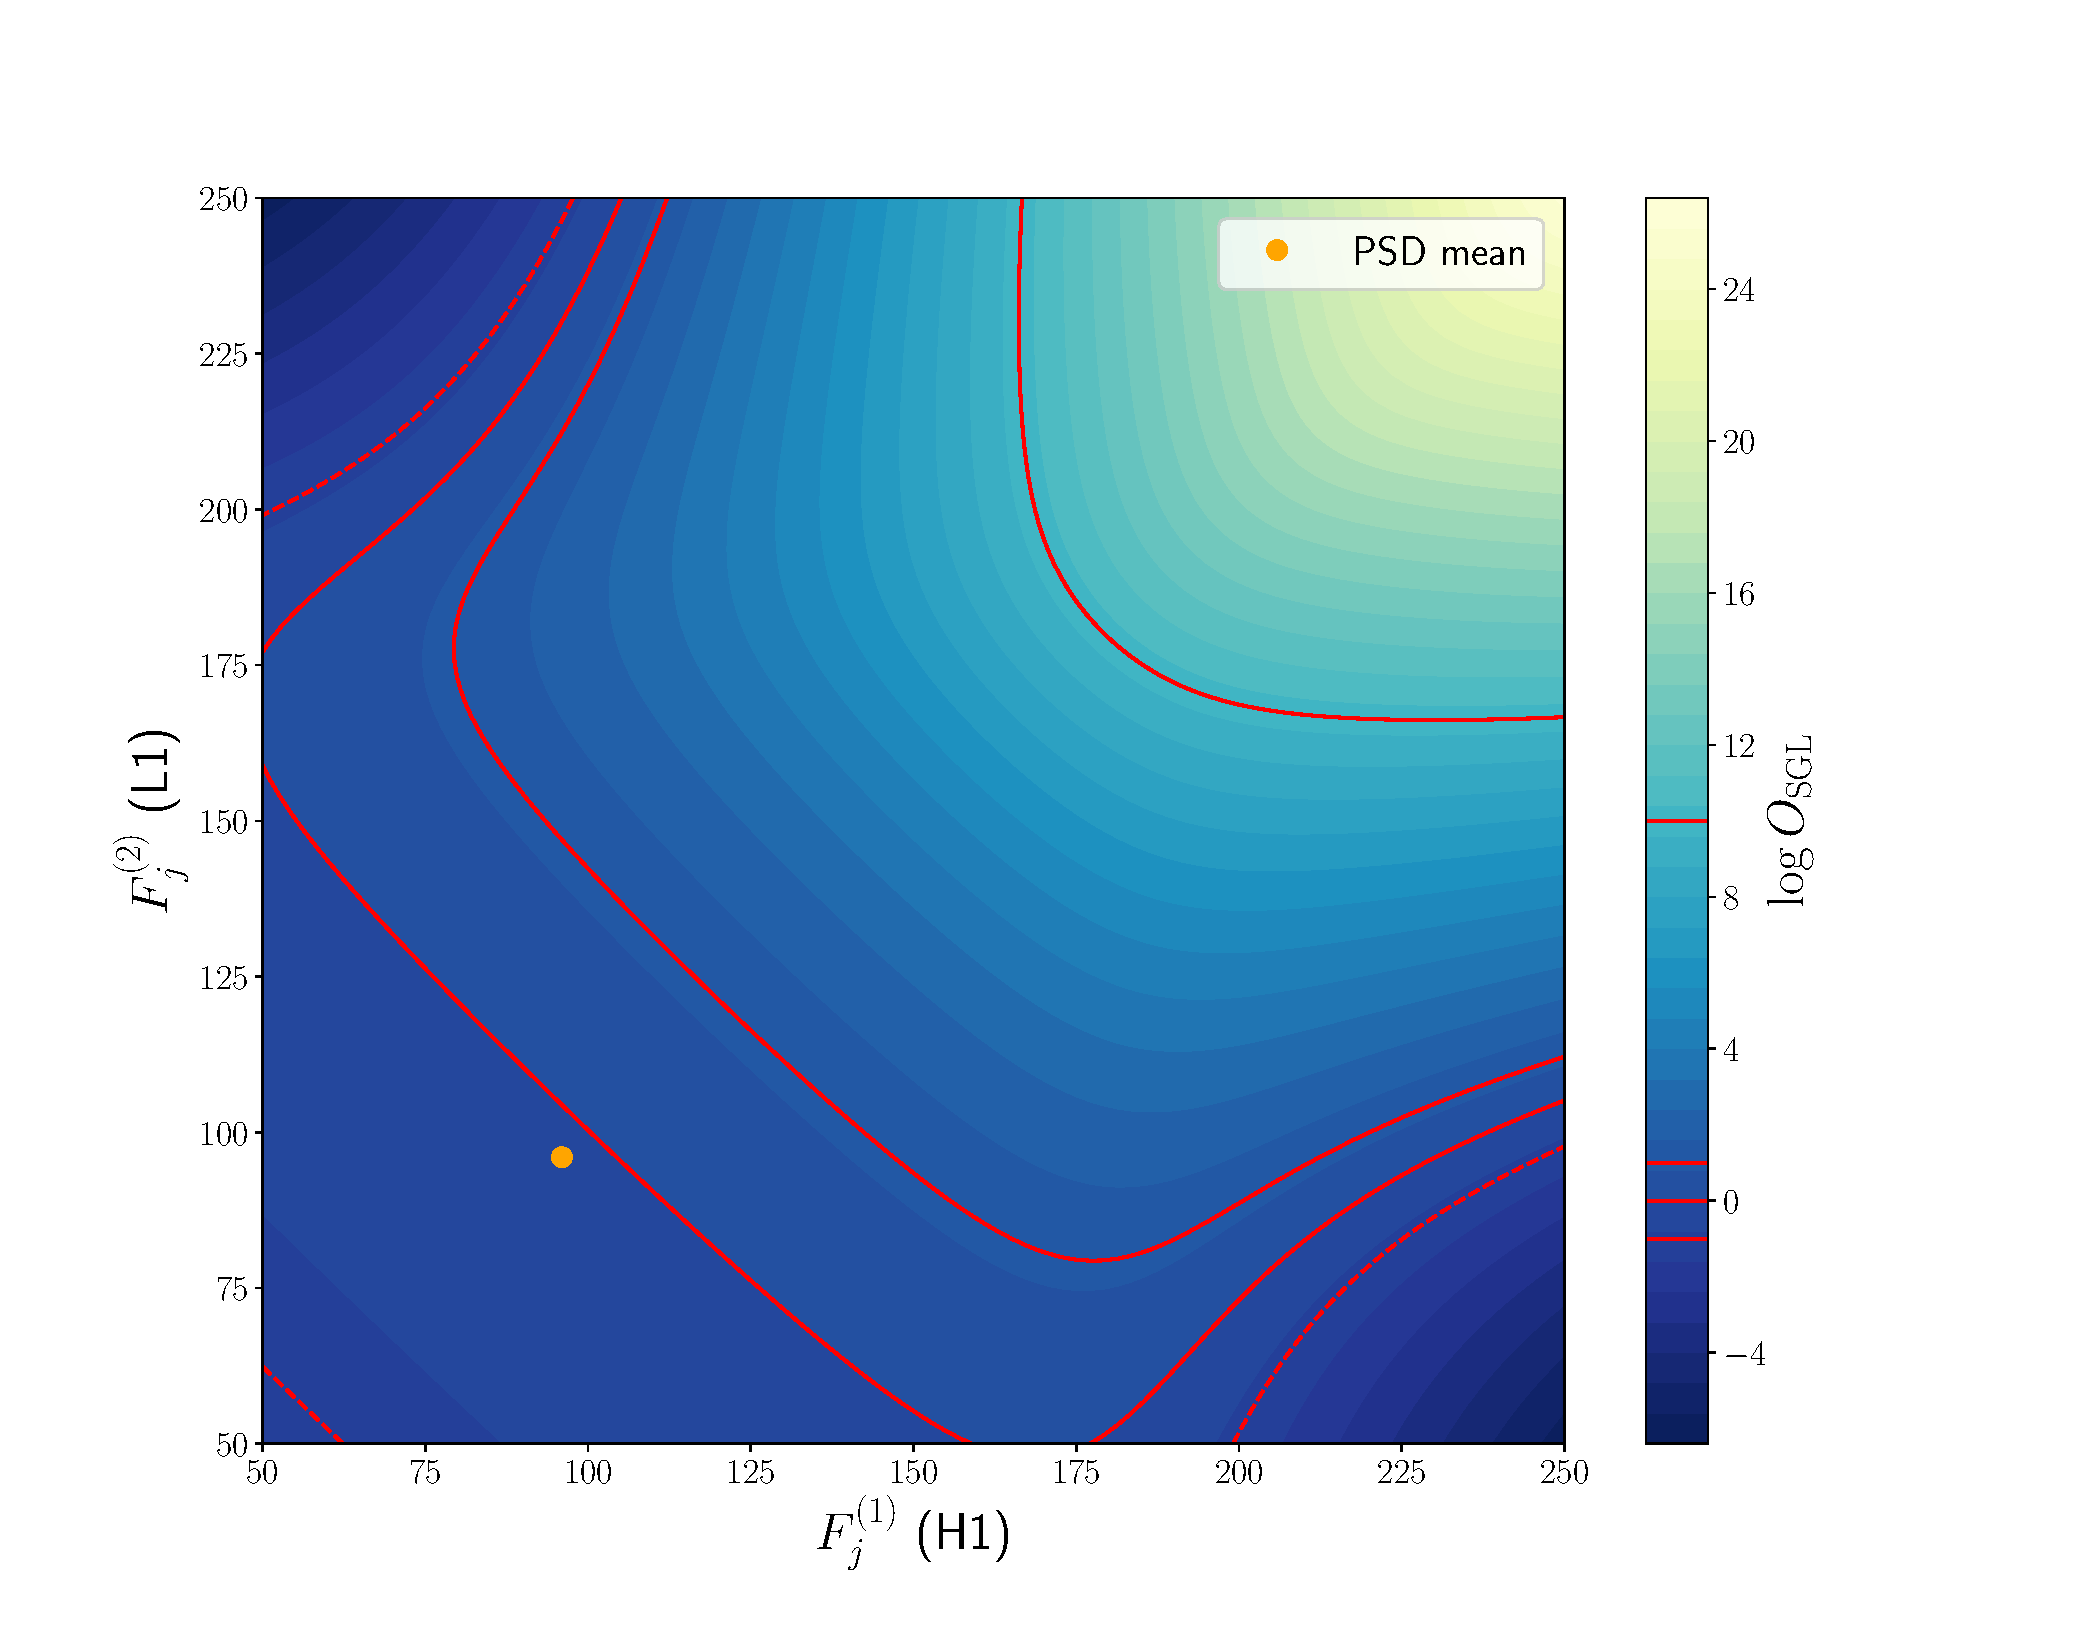
\includegraphics[width=1.\columnwidth]{lookup_linesmall.pdf}
\end{minipage}\hfill
\begin{minipage}{0.35\linewidth}
\caption{This shows the distribution of the lines aware statistic plotted against the \ac{FFT} power in each detector. This example is for parameters $p_s(\lambda) = 2$,$p_l(\lambda) = 2$ and $p(M_L)/p(M_G) = 1$. Here the line part of the statistic has the same \ac{SNR} and the signal part, i.e. we expect the \ac{SNR} of a signal to be similar to that of a line.}
\label{viterbi:plot:data}
\end{minipage}
\end{subfigure}

\begin{subfigure}[h]{\linewidth}
\begin{minipage}{0.65\linewidth}
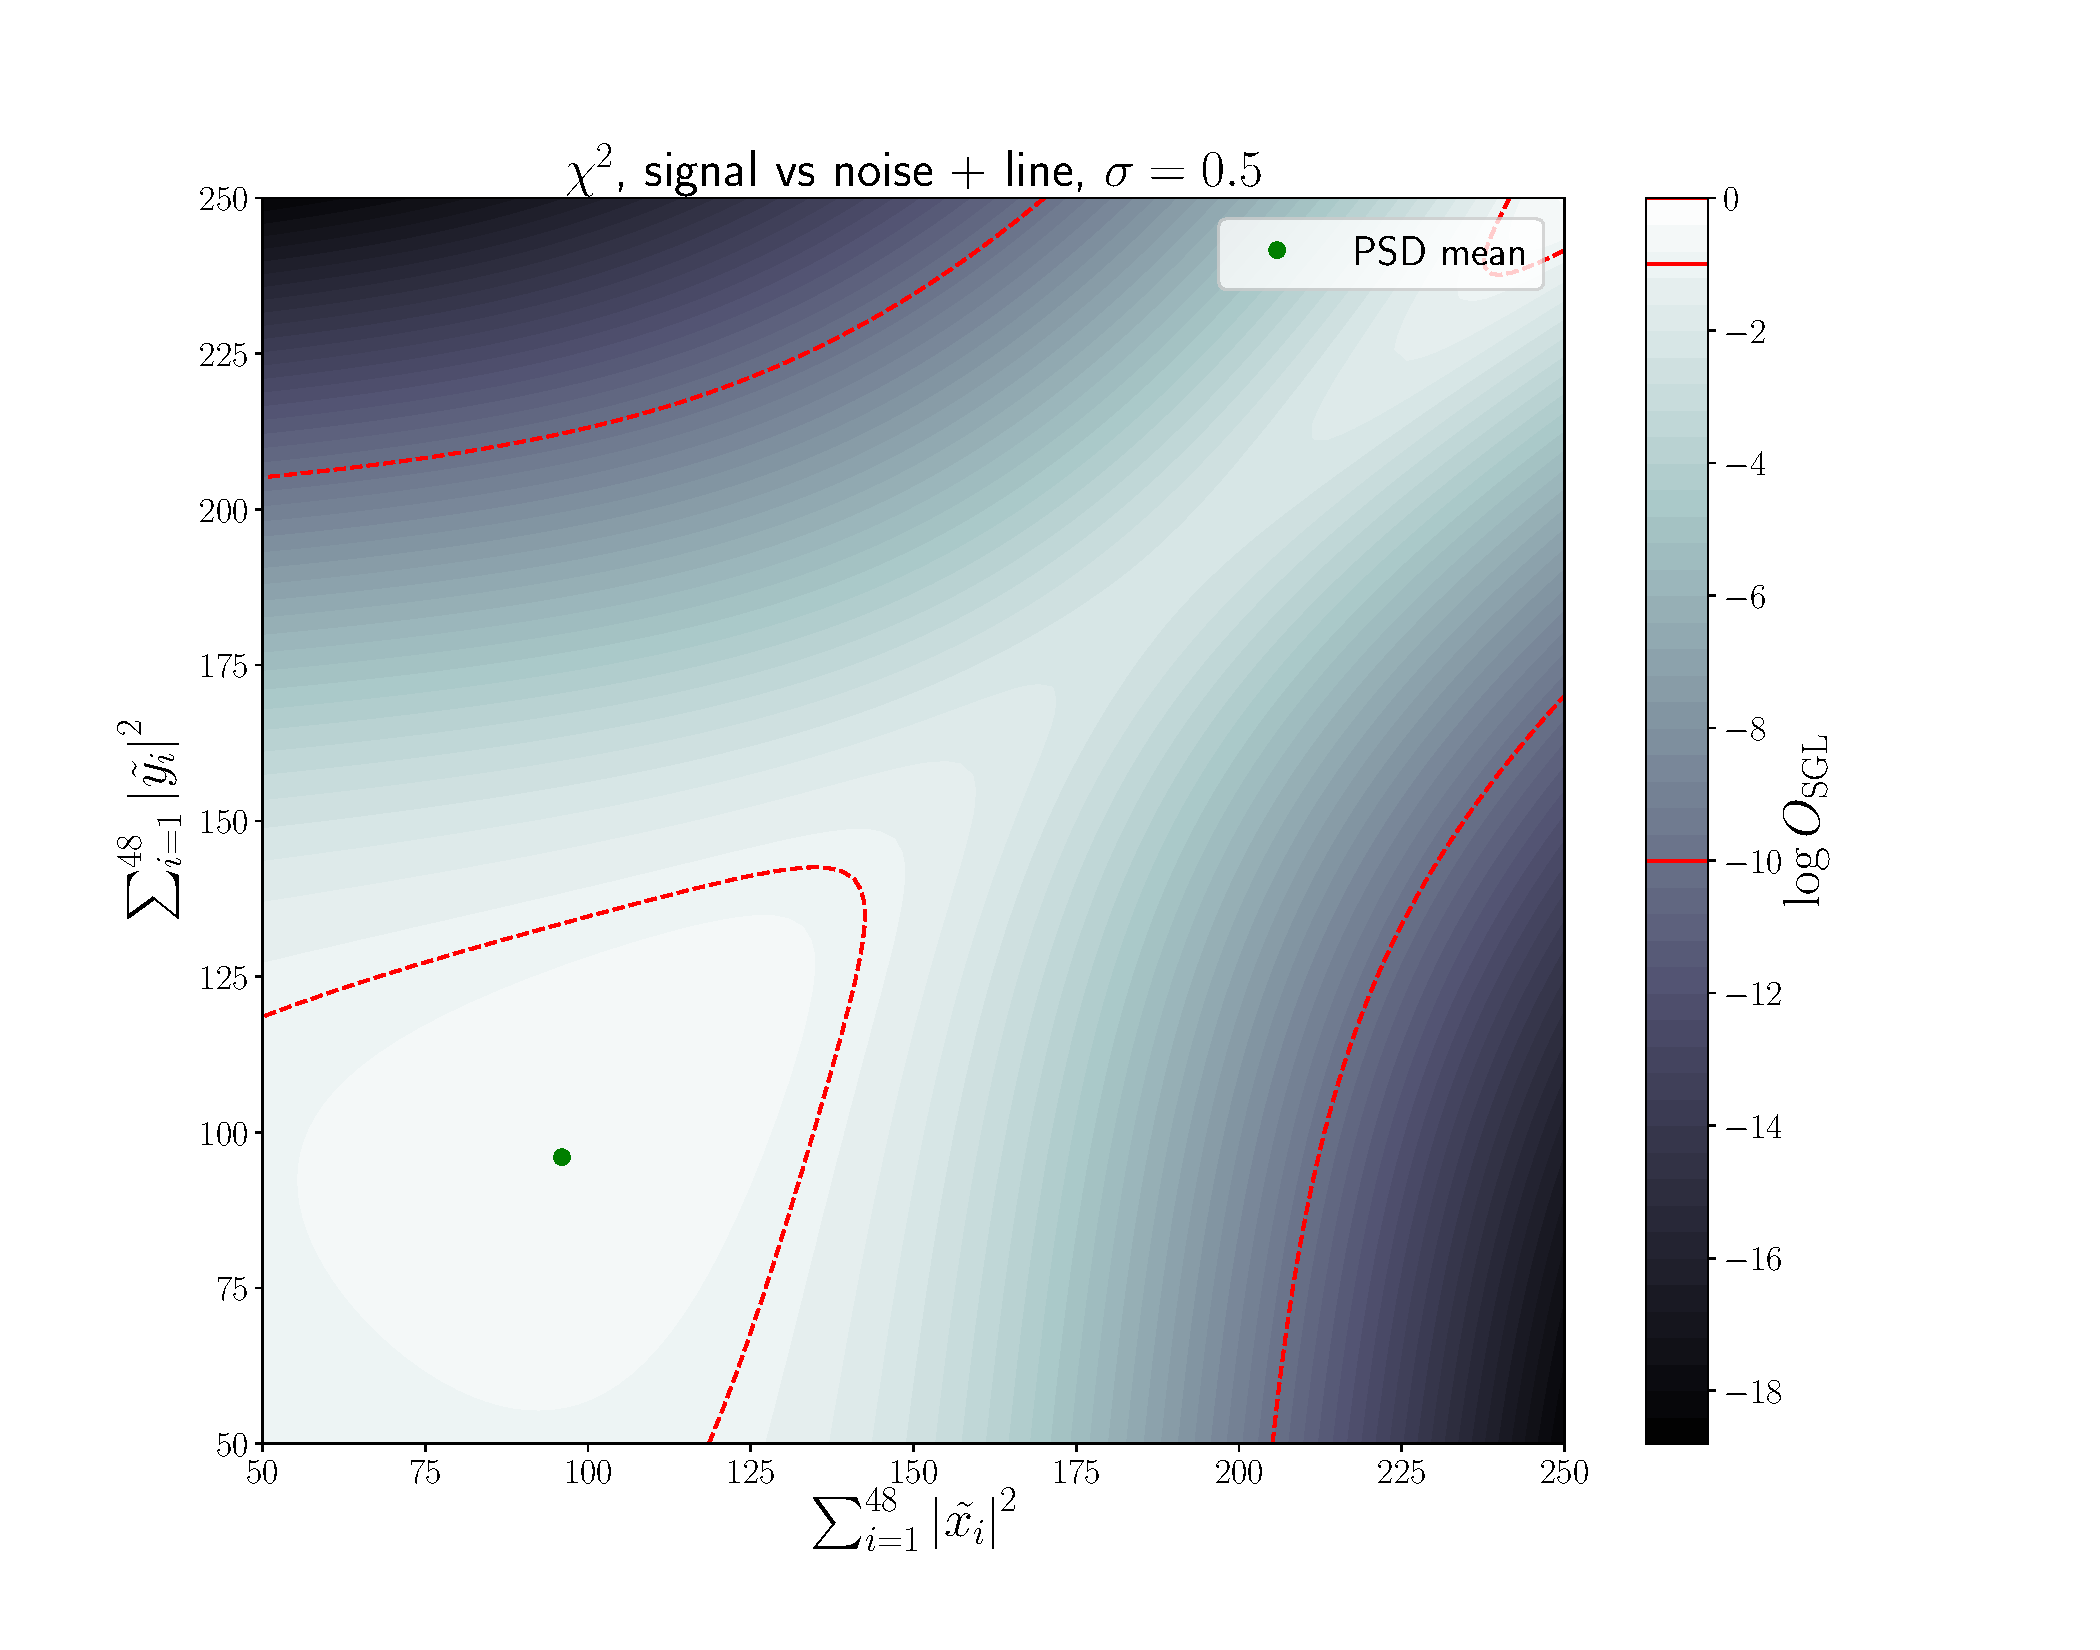
\includegraphics[width=1.\columnwidth]{lookup_linebig.pdf}
\end{minipage}\hfill
\begin{minipage}{0.35\linewidth}
\caption{This shows the distribution of the lines aware statistic plotted against the \ac{FFT} power in each detector. This example is for parameters $p_s(\lambda) = 2$,$p_l(\lambda) = 10$ and $p(M_L)/p(M_G) = 1$. Here we expect the \ac{SNR} of a line to be larger than a signal.}
\label{viterbi:plot:data}
\end{minipage}
\end{subfigure}
\caption{Lookup tables using the line aware statistic in Eq.~\ref{viterbi:las:logodds}.}
\label{viterbi:plots}
\end{figure}

